\section {Introduction}

Many of the searches for \charginopm and \neutralinotwo in ATLAS \cite{Aad:2012hba, ATLAS:2012ab} and CMS \cite{Chatrchyan:2012mea} involves events with three leptons and \met. Those searches dealt with some difficulties. Firstly with the increasing LHC luminosity both experiments needed to raise the \pt thresholds on the triggered objects with a consequent lowering of signal efficiency. Second Drell-Yan production of sleptons has a steep fall with the increase in invariant mass \cite{Baer:1997nh}.

As shown in early studies, however, an analysis of the \charginopm / \neutralinotwo system from a different angle  in Vector Boson Fusion (VBF) events is also possible \cite{Bjorken:1992er}. VBF production is characterized by the presence of two jets with a large di-jet invariant mass in the forward region in opposite hemispheres. Additionally the produced \charginopm and \neutralinotwo decay into multiple $\tau$ leptons and a \neutralinoone which travels through the detector undetected increasing \met. A sample diagram of \charginopm / \neutralinotwo pair production from VBF processes is shown in Figure \ref{fig:VBF_diagrams}. 

\begin{figure}[tbh!]
	\centering
	\begin{tabular}{cc}
		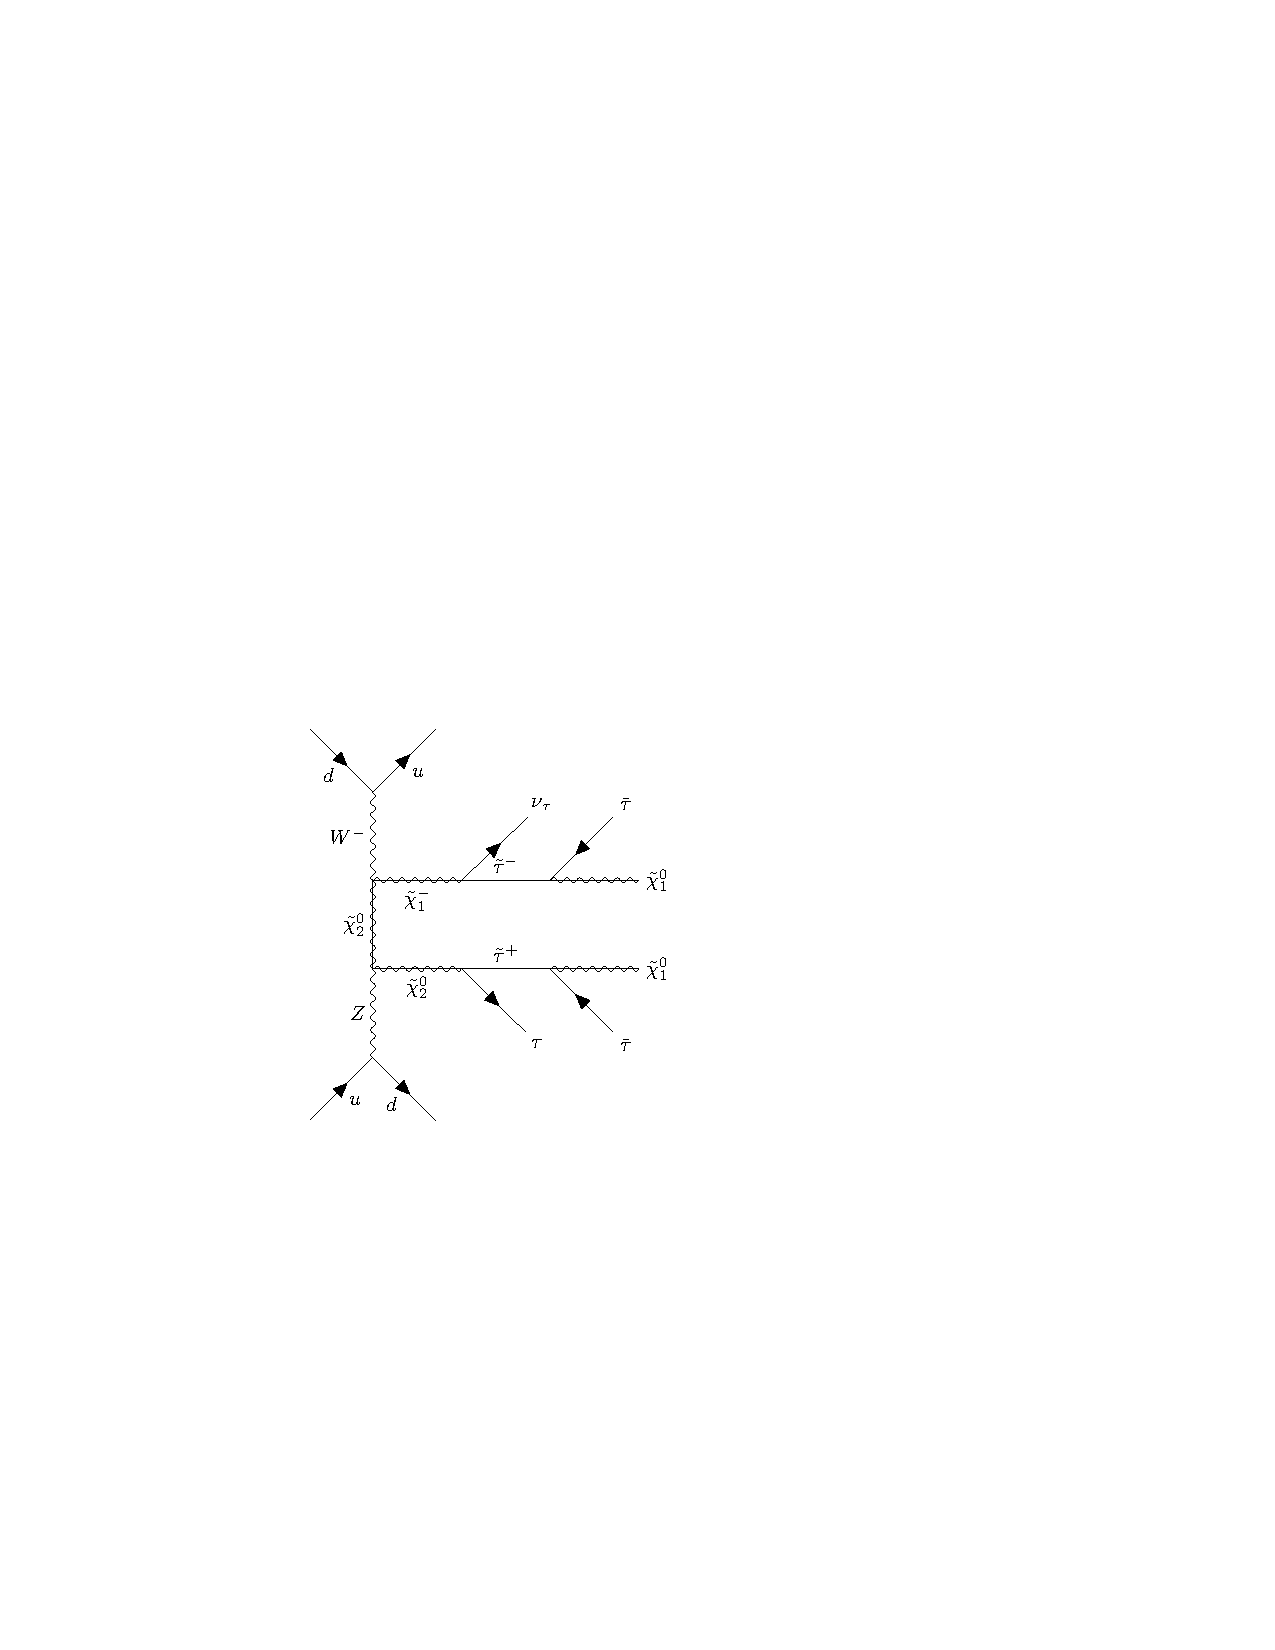
\includegraphics[width=0.48\textwidth]{diagrams/pics/signal_C1N2.pdf}
		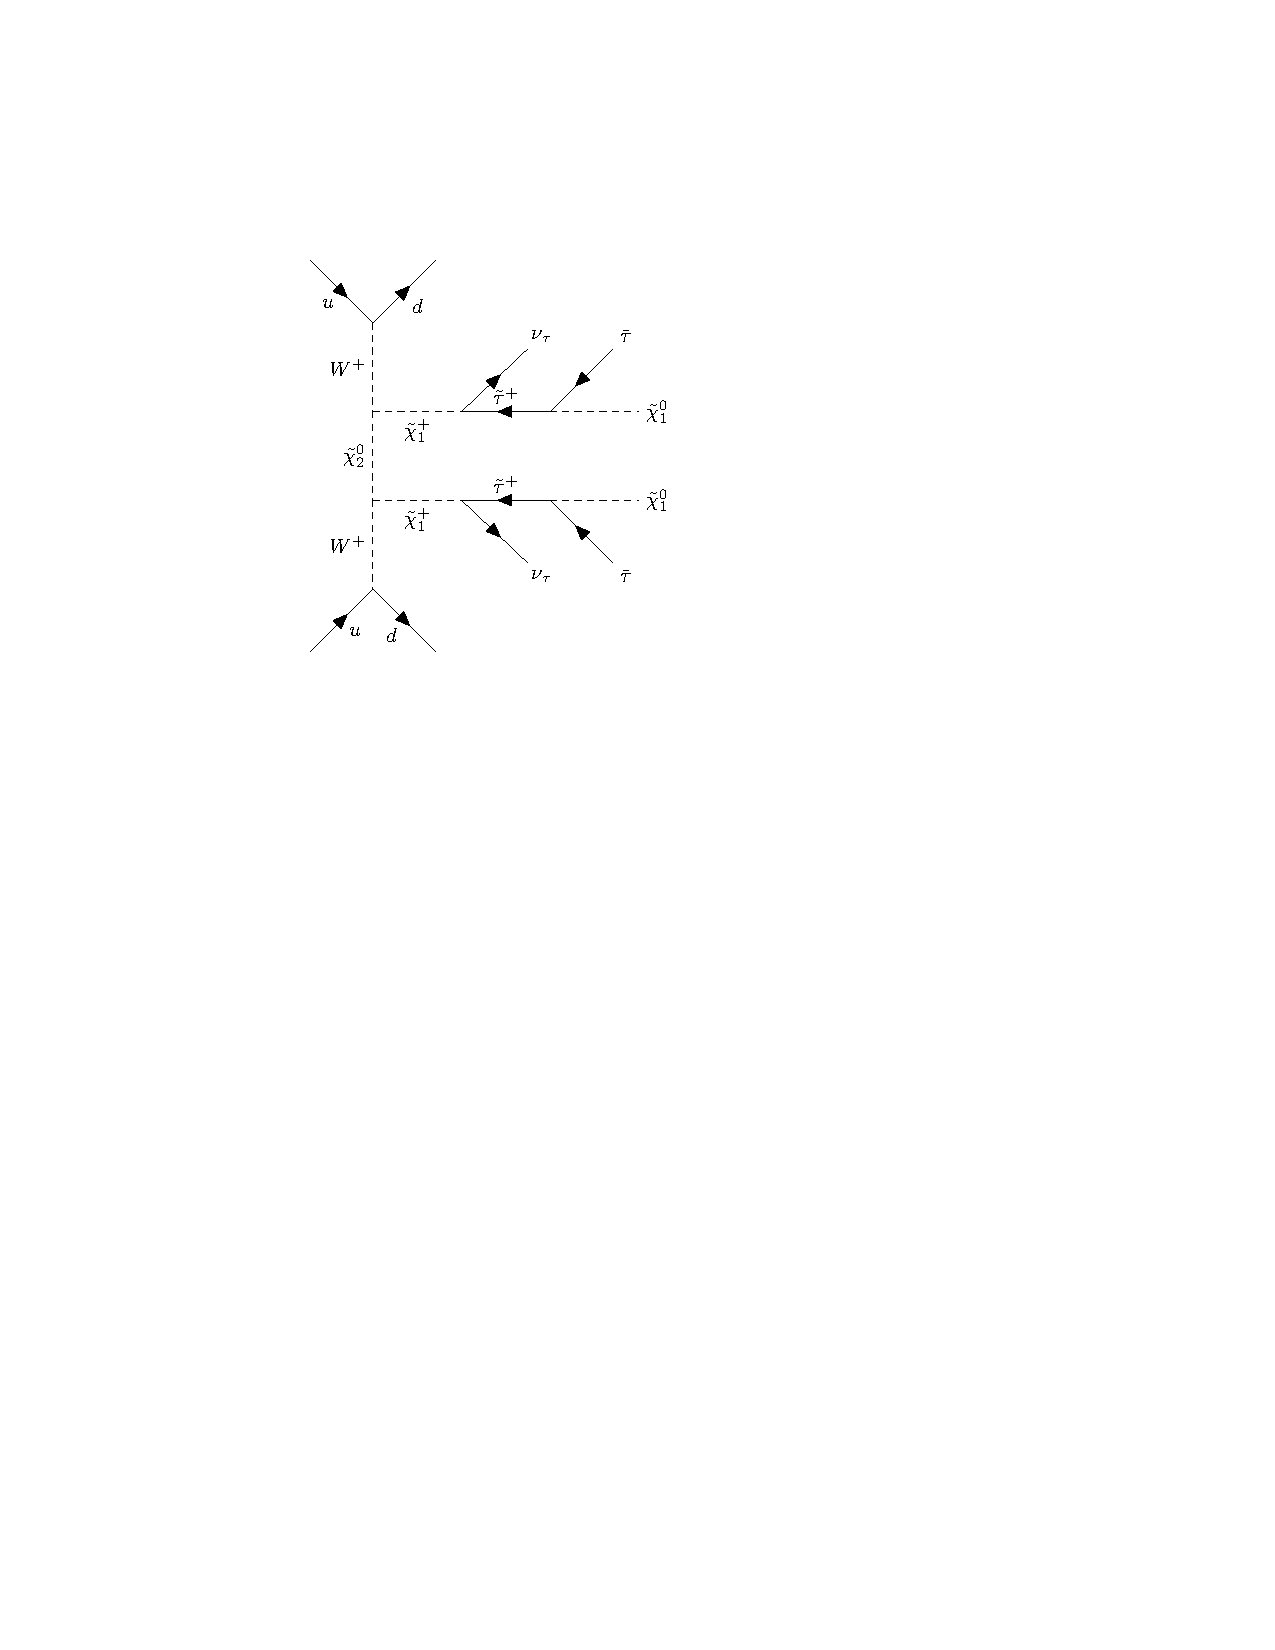
\includegraphics[width=0.48\textwidth]{diagrams/pics/signal_C1C1.pdf} 		
	\end{tabular}
	\caption{Diagrams of (left) \charginopm \neutralinotwo and (right) \charginopm \charginomp pair production through vector-boson fusion followed by their decays to $\tau$ leptons and the LSP.}
	\label{fig:VBF_diagrams}
\end{figure}

\section{VBF with two leptons and two jets}

This search for SUSY events with two leptons and two jets comes with some advantages with respect to the previous ones \cite{Dutta:2012xe}. First there is the possibility to probe signal for SUSY by triggering over the VBF properties of the event, leaving the decay products of \charginopm and \neutralinotwo free from online kinematic constraints.

Second VBF production allows the investigation of final states with $\tau$ leptons. This can be of advantage for SUSY scenarios with high \tanbeta, where the \stau is typically lighter than  \smuon and \selectron  \cite{Hinchliffe:1999zc}. A light \stau with small mass splitting is favored in coannihilation processes \cite{Griest:1990kh} that set the relic density to correct values, in the case of Bino dark matter. A light \stau is also motivated in the context of the MSSM by the enhancement of the $H \longrightarrow \gamma\gamma$ channel \cite{Carena:2011aa}. These facts stress the importance of searches in $\tau$ final states with low \pt and large backgrounds, for which production by VBF processes is more suited since the VBF signature allows for the reduction of the backgrounds to manageable levels.

Finally, Drell-Yan production cross-section falls faster than the VBF production cross-section with increasing mass allowing further control over background distributions \cite{Datta:2002vy} .

The main feature of VBF processes is the production of a jet pair aimed at the forward-backward region of the detector with high \pt and large \deltaeta. By adding to the event selection the requirements on the di-jet \deltaeta as well as the di-jet invariant mass \ensuremath{m_{j_{1}j_{2}}} the background contribution coming from V+jets and \ttbar events, shown in Figures \ref{fig:background_W3jets} and \ref{fig:background_ttbar}, is kept under control. In order to generate supersymmetric particles, the incoming partons need to have an high momentum, so that the leading jet from the VBF-produced di-jet pair is expected to have high \pt. The addition of a \pt cut on leading jets further reduces background contributions. Figure \ref{fig:VBF_mjj_ptj1} shows a study on \ensuremath{m_{j_{1}j_{2}}} and leading jet \pt distributions for \charginopm \charginopm pair production by VBF processes, V+jets background, and VV background produced by VBF processes for \ensuremath{m_{\charginopm} = m_{\neutralinotwo} = 300, 200} and \ensuremath{100\gev}, \ensuremath{m_{\charginopm} - m_{\tilde{\tau}} = 5\gev} and \ensuremath{m_{\neutralinoone} = 0\gev}.

The remaining background contributions come from all the centrally produced particles. By considering an R-parity conserving model the decay of \charginopm and \neutralinotwo is the following

\begin{equation}
\charginopm \longrightarrow \stau^{\pm} \nu \longrightarrow \tau^{\pm} \neutralinoone \nu ;
\end{equation}

\begin{equation}
\neutralinotwo \longrightarrow \stau^{\pm} \tau^{\mp} \longrightarrow \tau^{\pm} \tau^{\mp} \neutralinoone.
\end{equation}

Processes with same signature are all the VV (where V may be both W or Z) pairs produced via VBF where the bosons decays leptonically. Furthermore, in case of \hadtau decays Quantum Chromo Dynamics (QCD) multijet becomes the most appreciable background contribution. A \met cut is effective in reducing those backgrounds as shown on Figure \ref{fig:VBF_met_pttau}. Requiring multiple $\tau$’s in the event further reduces background. The \pt of the \ensuremath{\tau} coming from the \charginopm and \neutralinotwo decays is strongly correlated to the mass difference between the \charginopm and the \neutralinoone LSP. In Figure \ref{fig:VBF_met_pttau}, the normalized distribution of the \pt of \ensuremath{\tau} is displayed for \ensuremath{m_{\charginopm} = m_{\neutralinotwo} = 300\gev}, \ensuremath{m_{\charginopm} - m_{\tilde{\tau}} = 5\gev} and \ensuremath{m_{\neutralinoone} = 0\gev}. For smaller \ensuremath{\Delta M}, the distribution peaks at lower \pt and the signal acceptance is less efficient.

\section {Search Strategy}
\label{section::search_strategy}

For this type of search several benchmark points are defined under the following constraints. Firstly the \charginopm and \neutralinotwo are mainly Wino-like, while the \neutralinoone is mainly Bino-like. Furthermore the \charginomp mass similar to the \neutralinotwo mass ($m_{\charginopm} \sim m_{\neutralinotwo}$) and with values of 100, 200 and 300\gev. Additionally the mass gap between the \stau and \charginopm is either 5 \gev or $(m_{\stau} - m_{\charginopm})/2$. Finally The LSP mass is either $\neutralinoone = 0$, or 50\gev.

The processes taken into account are

\begin{equation}
pp \longrightarrow \charginopm \charginomp jj, \quad pp \longrightarrow \charginopm \neutralinotwo jj, \quad pp \longrightarrow \neutralinotwo \neutralinotwo jj
\end{equation}

The cross-section prediction for each of those processes are shown in Figure \ref{fig:VBF_xsec} as function of the \charginomp - \neutralinotwo mass.

\begin{figure}[tbh!]
	\centering
	\begin{tabular}{cc}
		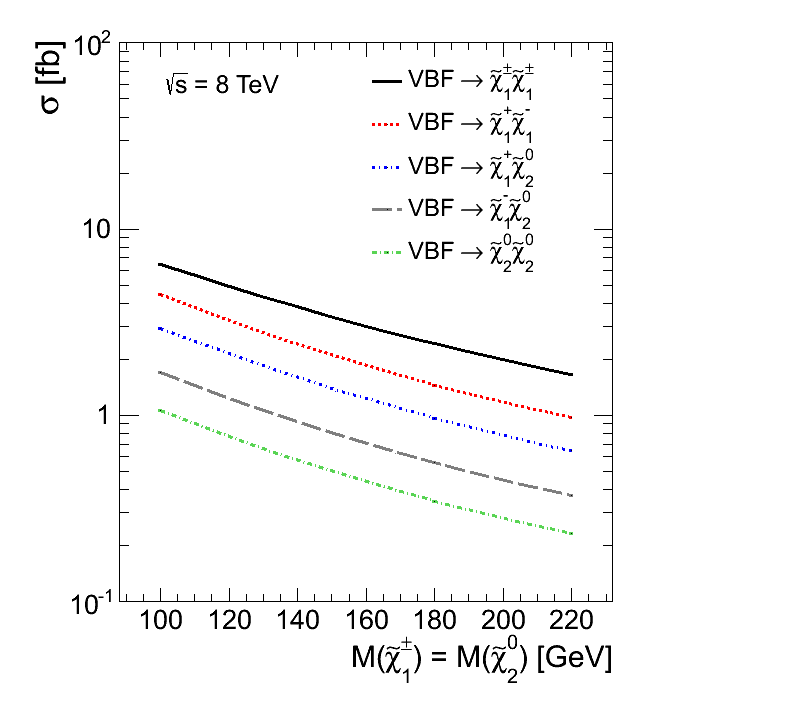
\includegraphics[width=0.75\textwidth]{analysis/pics/VBFXsection.png}
	\end{tabular}
	\caption{VBF production cross-section at \CM = 8 \tev as a function of mass for various channels after imposing \ensuremath{\deltaeta > 4.2} using Madgraph 4 (NLO) \cite{Dutta:2012xe}.}
	\label{fig:VBF_xsec}
\end{figure}

The search strategy can be divided in two distinct parts: the first one considers the kinematic of the jets produced via VBF in order to reduce the contribution coming  from V + jets events (where V is ether the W or Z boson); the second one takes into account decay products of the supersymmetric particles falling into the inner region of the detector (centrally produced) in order to reduce the all background contributions.

\begin{figure}[tbh!]
	\centering
	\begin{tabular}{cc}
		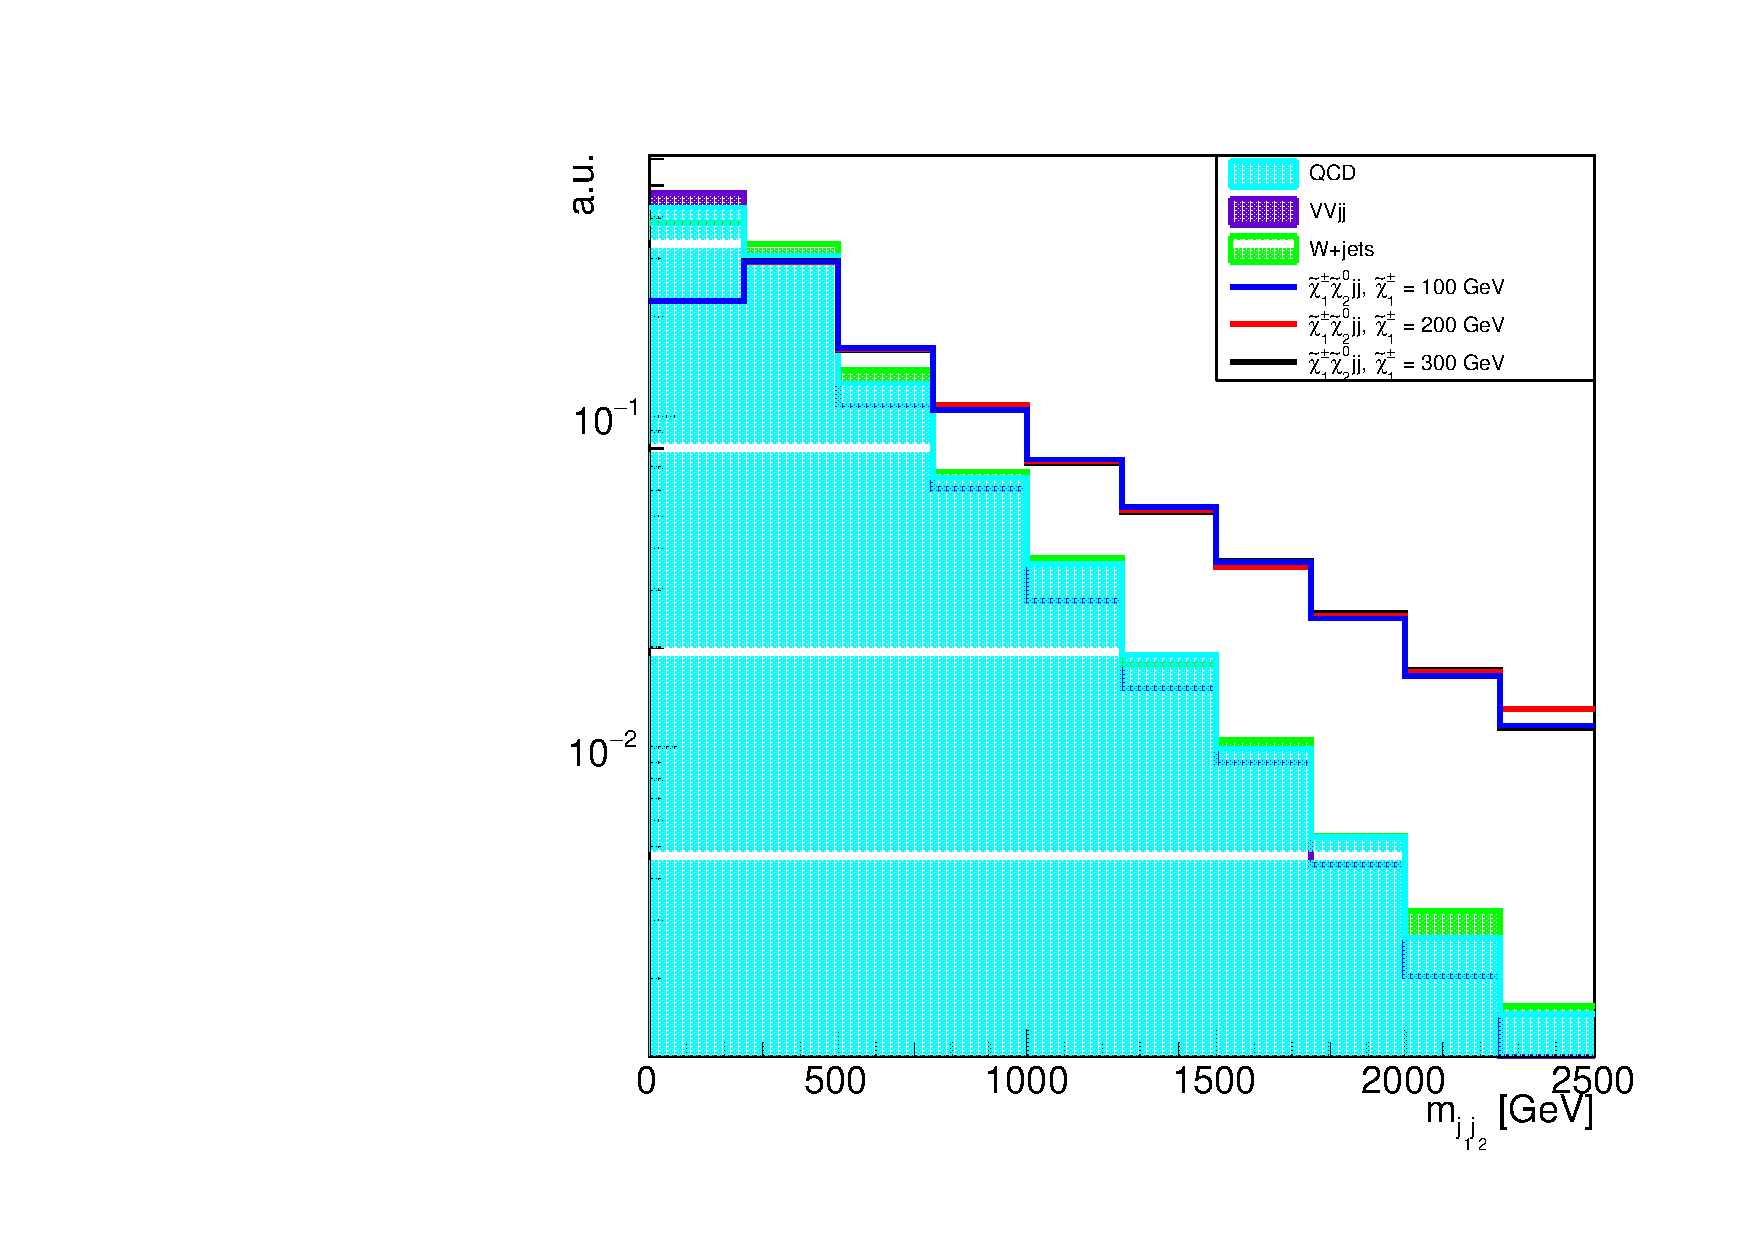
\includegraphics[width=0.48\textwidth]{analysis/pics/h_dijetinvariantmass_prospects13tev.pdf}
		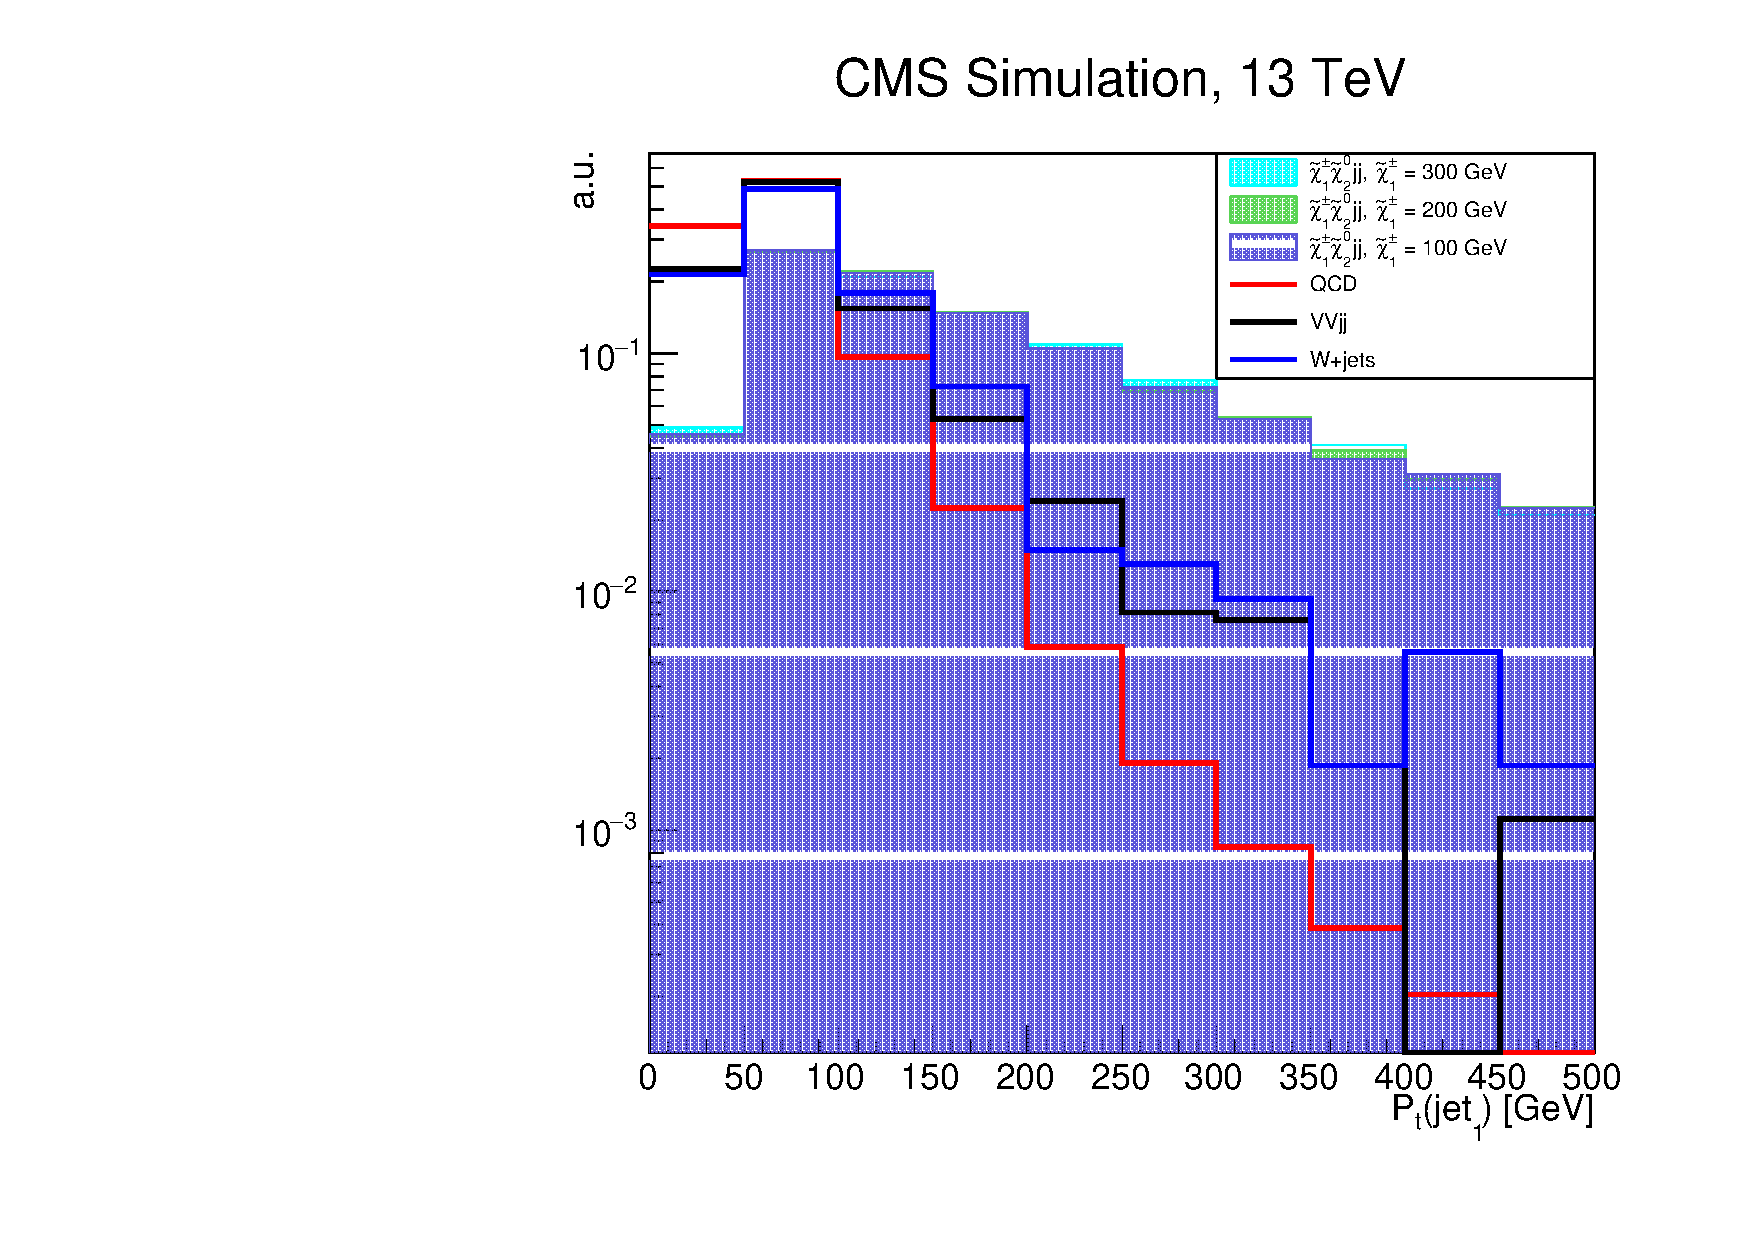
\includegraphics[width=0.48\textwidth]{analysis/pics/h_jet1pt_prospects13tev.pdf} 		
	\end{tabular}
	\caption{\ensuremath{m_{j_{1}j_{2}}} (left) and \pt of the leading jet (right) distributions normalized to arbitrary units for \charginopm \charginopm pair production by VBF processes, V+jets background, and VV background produced by VBF processes and QCD processes. The chosen signal benchmark point features \ensuremath{m_{\charginopm} = m_{\neutralinotwo} = 300, 200} and \ensuremath{100\gev}, \ensuremath{m_{\charginopm} - m_{\tilde{\tau}} = 5\gev} and \ensuremath{m_{\neutralinoone} = 0\gev}.}
	\label{fig:VBF_mjj_ptj1}
\end{figure}

\begin{figure}[tbh!]
	\centering
	\begin{tabular}{cc}
		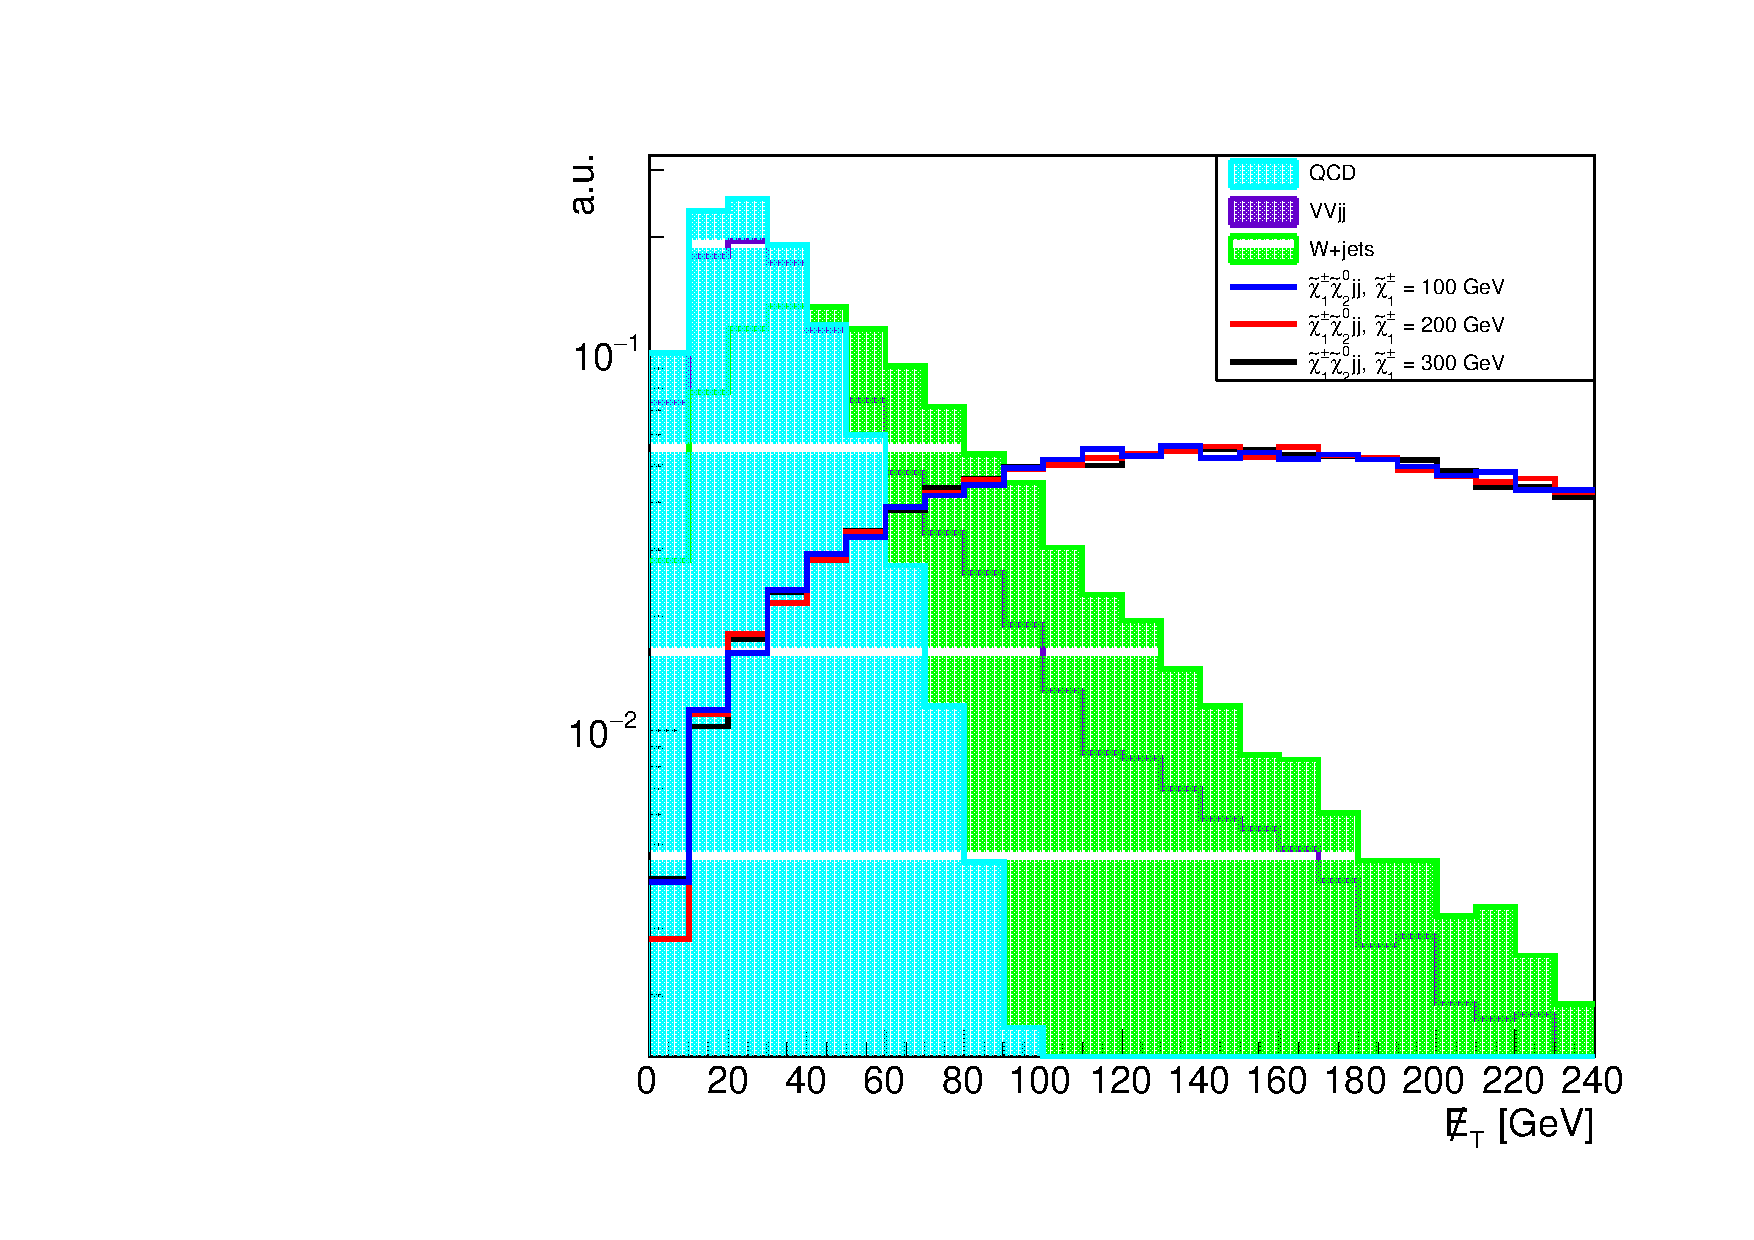
\includegraphics[width=0.48\textwidth]{analysis/pics/h_met_prospects13tev.pdf}
		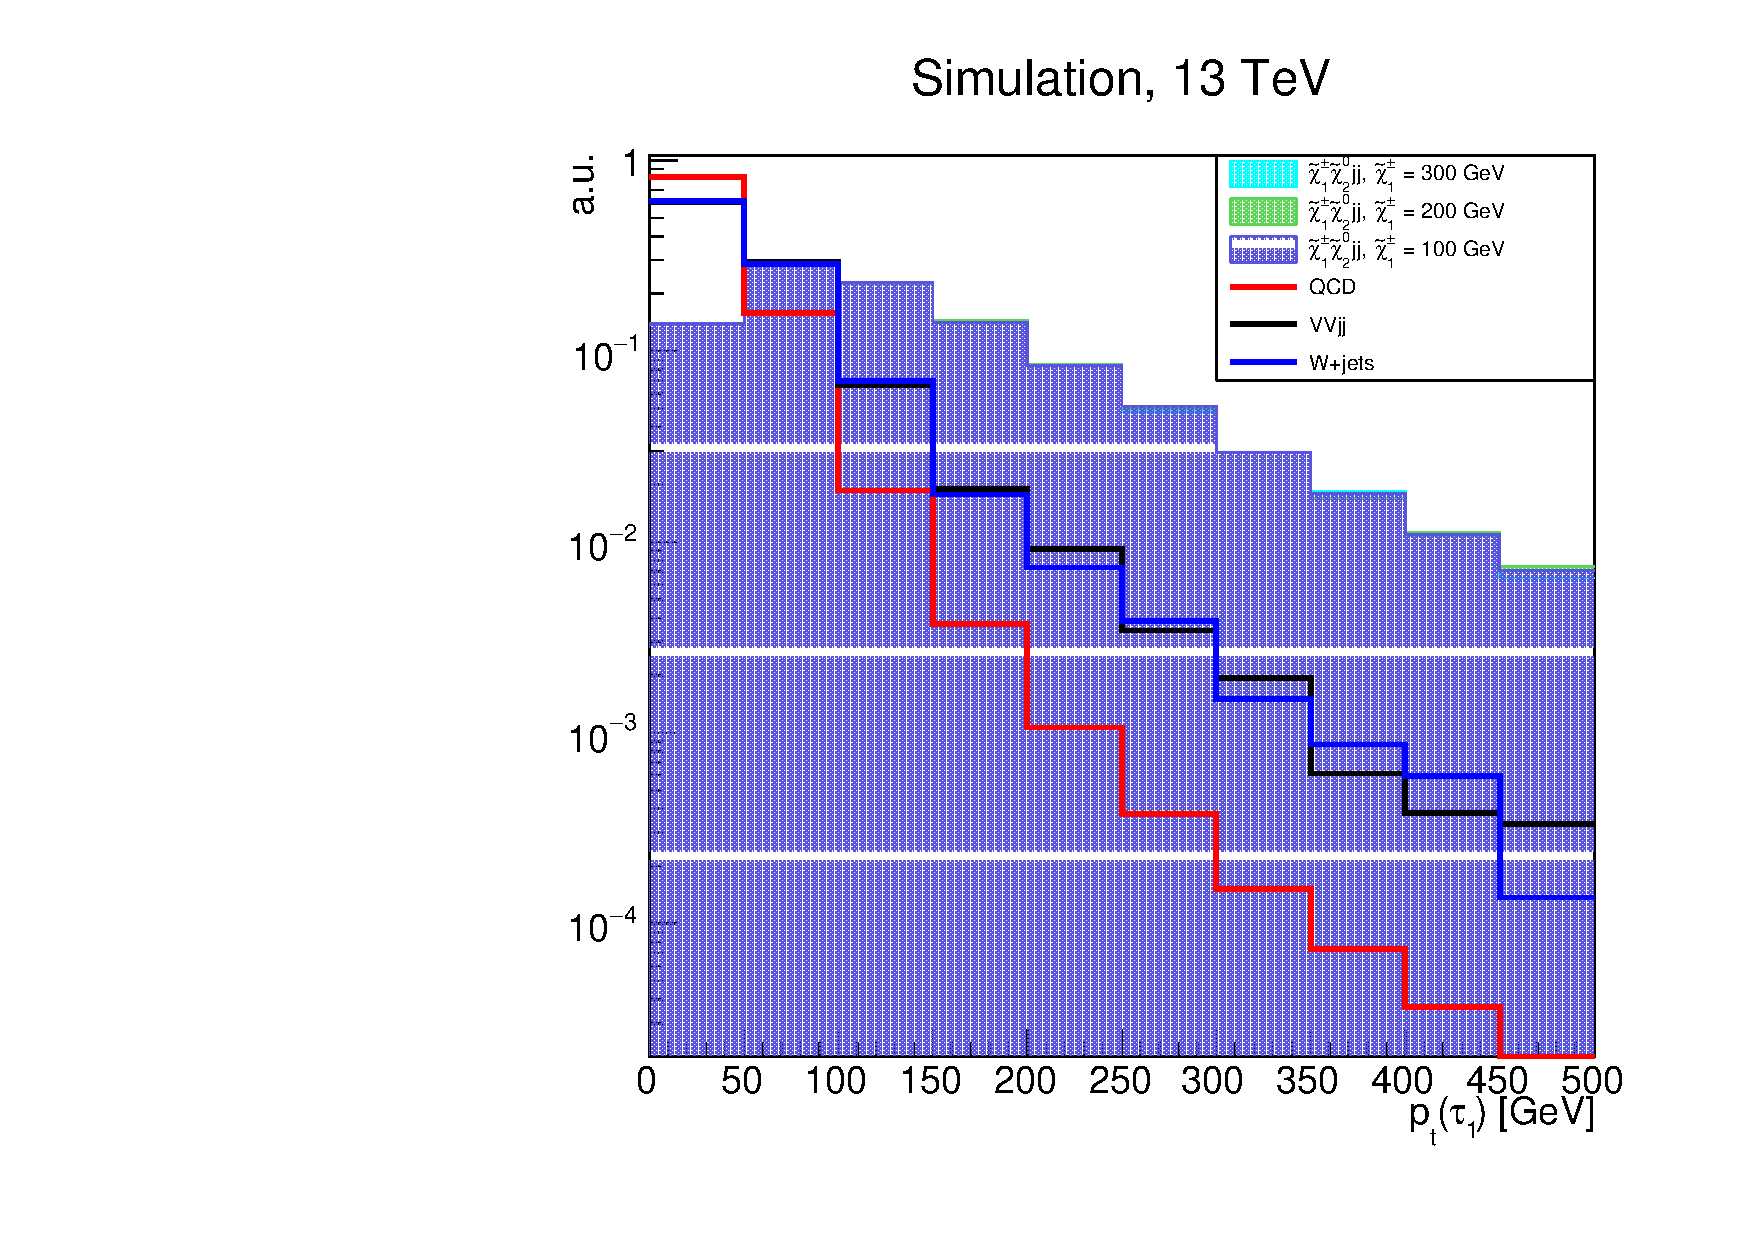
\includegraphics[width=0.48\textwidth]{analysis/pics/h_tau1pt_prospects13tev.pdf} 		
	\end{tabular}
	\caption{(left) \met and (right) leading \ensuremath{\tau} \pt distributions normalized to arbitrary units in \ensuremath{\geq 2j + 2\tau} final state for \charginopm \charginopm pair production by VBF processes, V+jets background, and VV background produced by VBF processes and QCD processes. The chosen signal benchmark point features \ensuremath{m_{\charginopm} = m_{\neutralinotwo} =300, 200} and \ensuremath{100\gev}, \ensuremath{m_{\charginopm} - m_{\tilde{\tau}} = 5\gev} and \ensuremath{m_{\neutralinoone} = 0\gev}.}
	\label{fig:VBF_met_pttau}
\end{figure}


\section{VBF with two same sign hadronic $\tau$ and two jets}

Besides the two oppositely directed forward jets that define the VBF configuration, the search requires the presence of at least two leptons coming from the different decay modes of the $\tau$ and large \met. The chosen search channels are $e\mu jj$, $\mu\mu jj$, $\mu\hadtau jj$, and $\hadtau\hadtau jj$. The final states are further differentiated into like-sign (LS) and opposite-sign (OS) di-lepton pairs for a total of eight different search channels. This thesis focuses its attention on the di-\hadtau LS channel search and its background estimation strategy. 


\section{Background Contributions}

The most important aspect of any search for new physics is the methodology used to estimate the background contribution in the signal region. The first step consists in the determination of all the irreducible background sources and the definition of an estimation technique for each of the contributions. Four types of background contributions have been considered in this analysis. 

The first irreducible background contribution is coming from the Standard Model VBF processes resulting in two \hadtau and two jets as shown in Figure \ref{fig:background_SMVBF}. This background contribution is well modeled being purely electroweak and its cross section is very small. Therefore this background is considered minor and its contribution is directly taken from simulation.

\begin{figure}[tbh!]
	\centering
	\begin{tabular}{cc}
		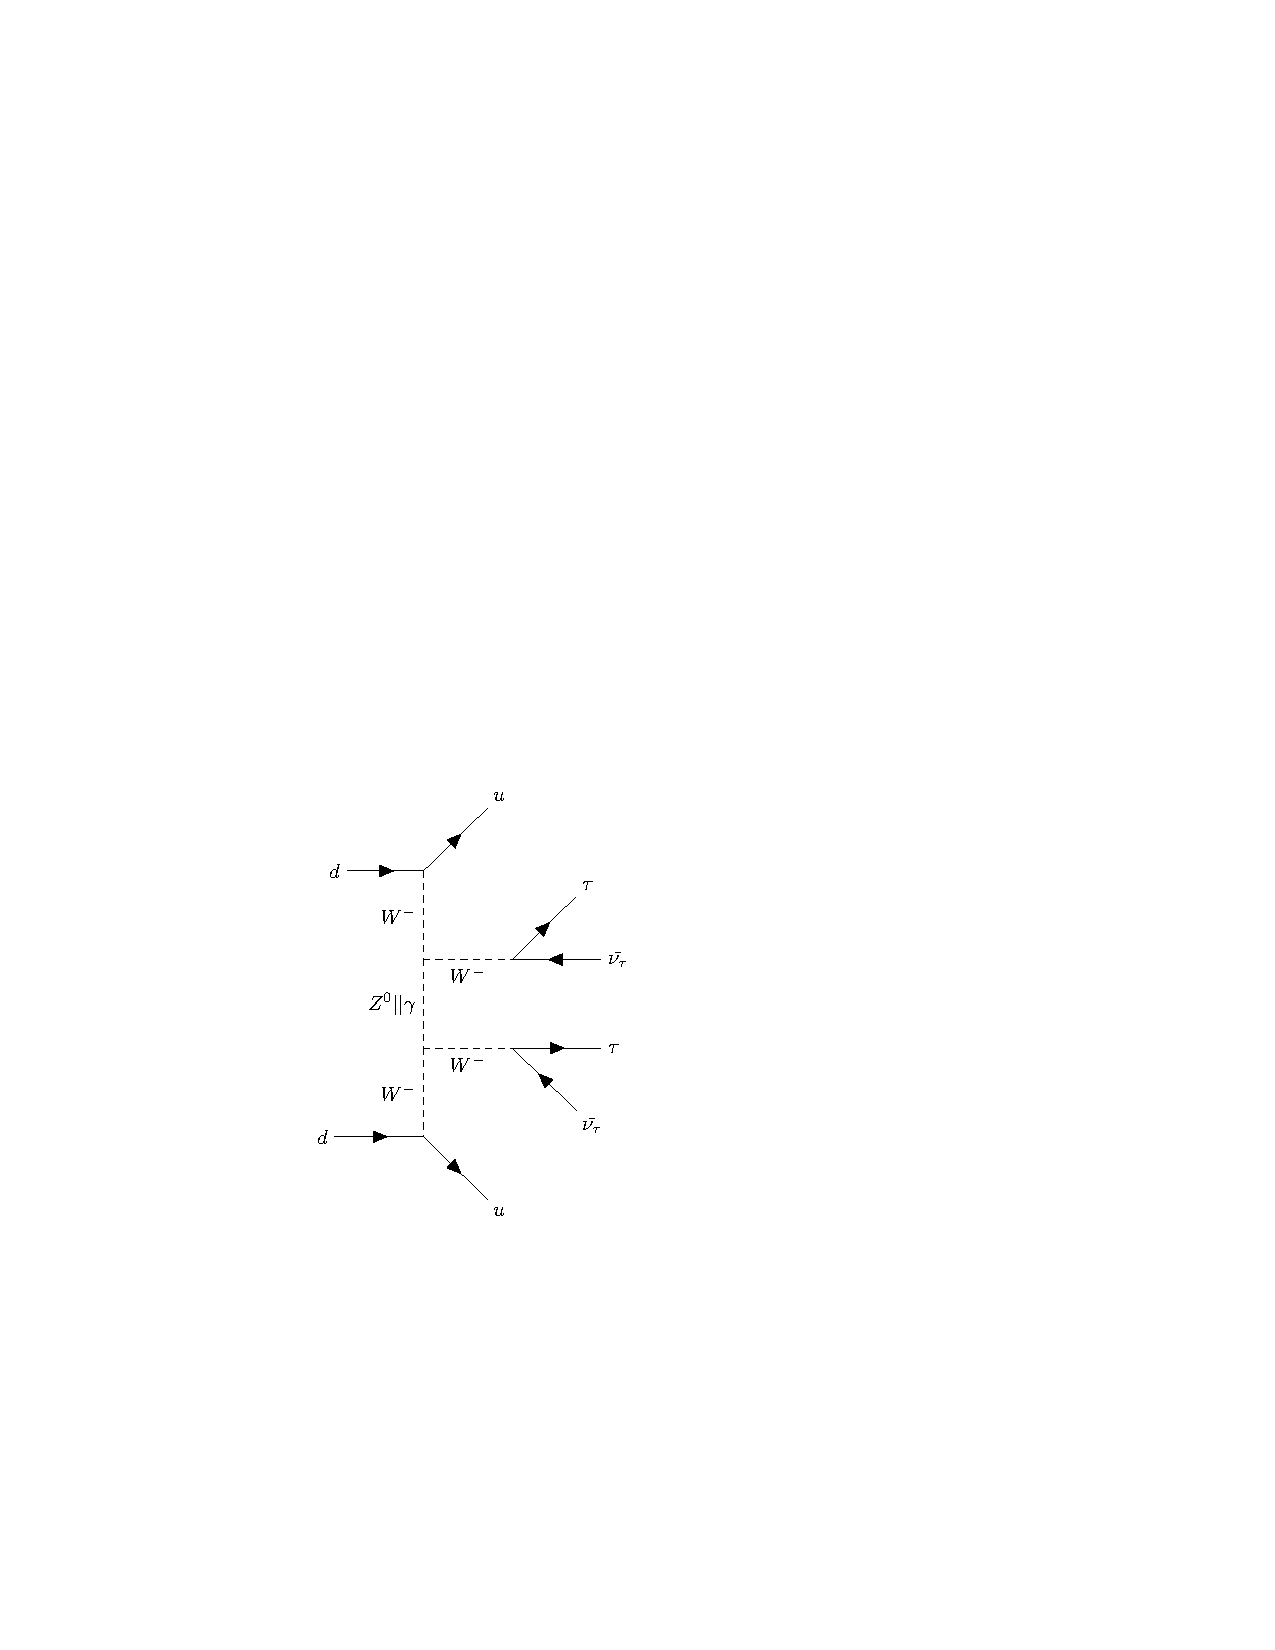
\includegraphics[width=0.48\textwidth]{diagrams/pics/background_SMVBFminus.pdf}
		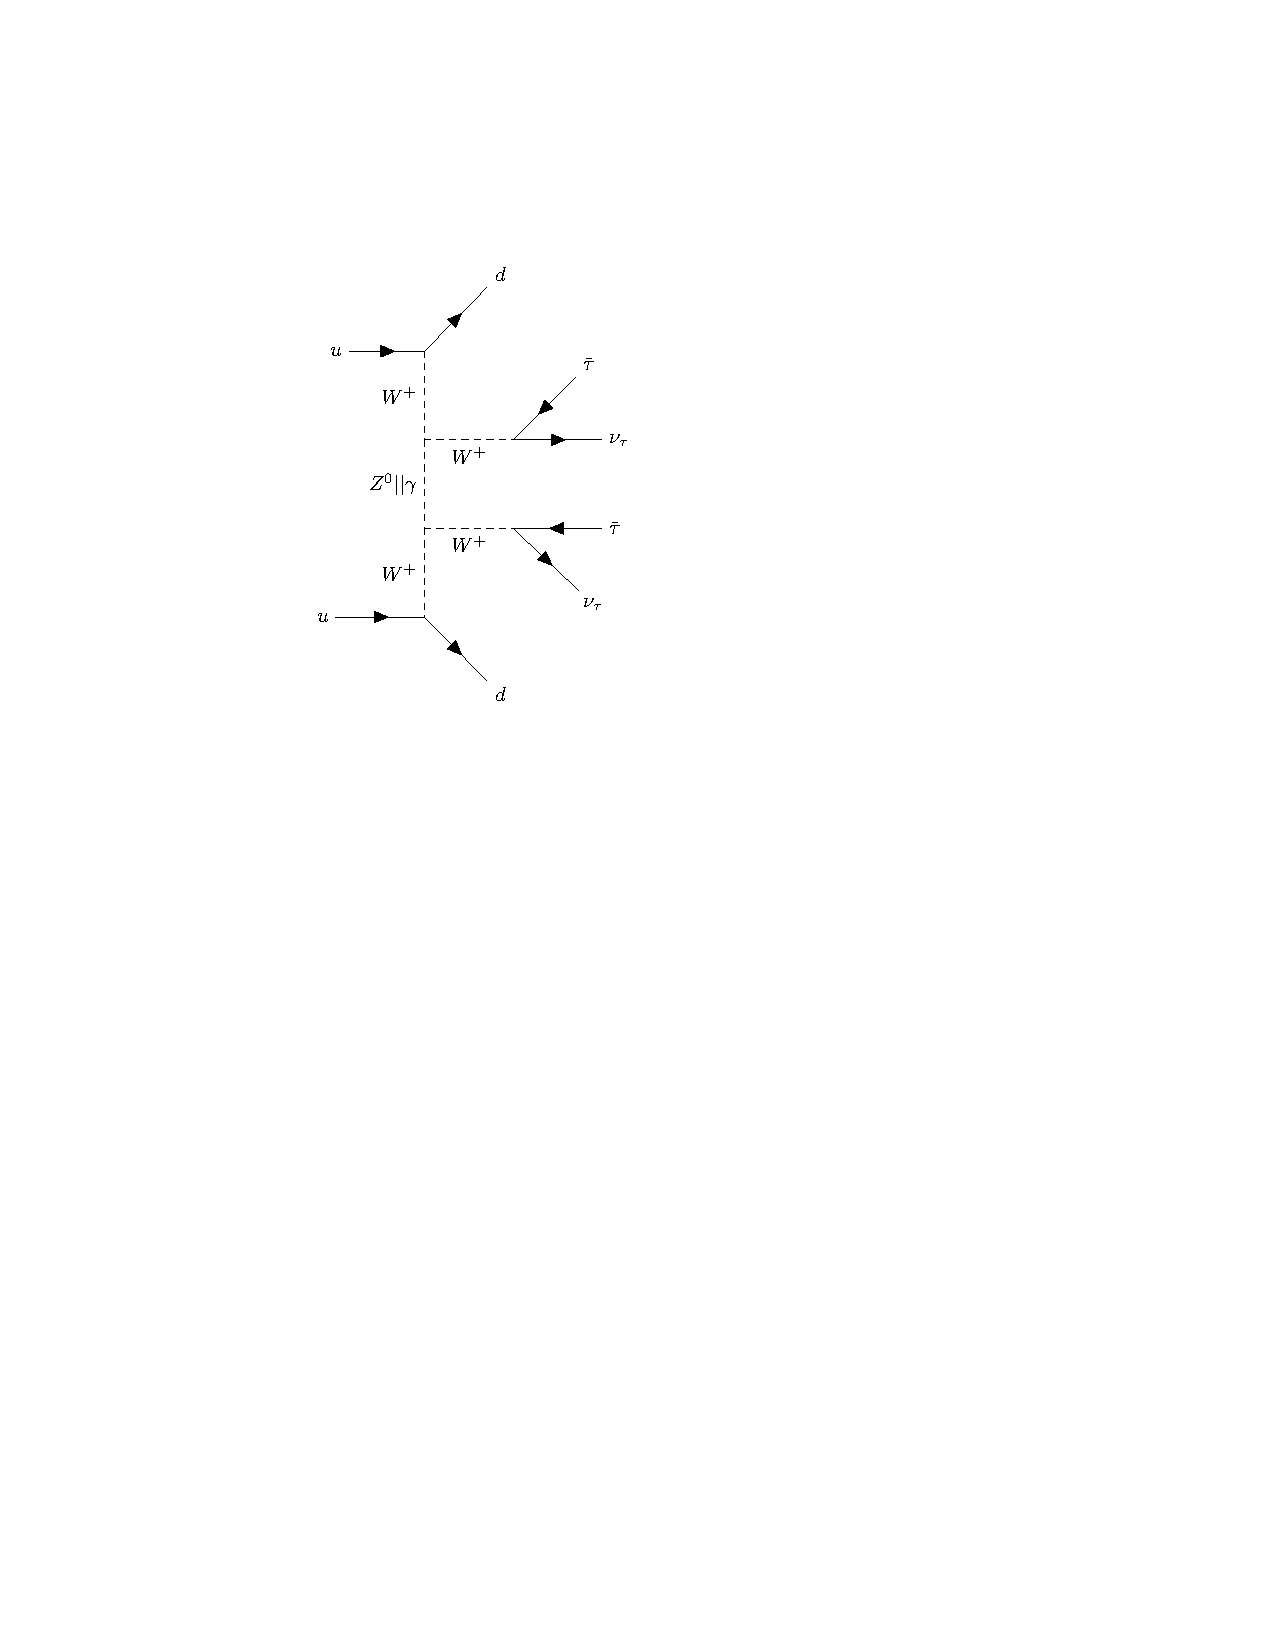
\includegraphics[width=0.48\textwidth]{diagrams/pics/background_SMVBFplus.pdf} 		
	\end{tabular}
	\caption{Feynman diagrams of irreducible backgrounds of Standard Model Vector Boson Fusion processes with two \hadtau and two jets final state. }
	\label{fig:background_SMVBF}
\end{figure}

Second, all the Standard Model VBF processes resulting in three leptons, with the opposite charged lepton, failing to pass the tauID, are considered as shown on \ref{fig:background_SMVBFZ0Wmiss}.

\begin{figure}[tbh!]
	\centering
	\begin{tabular}{cc}
		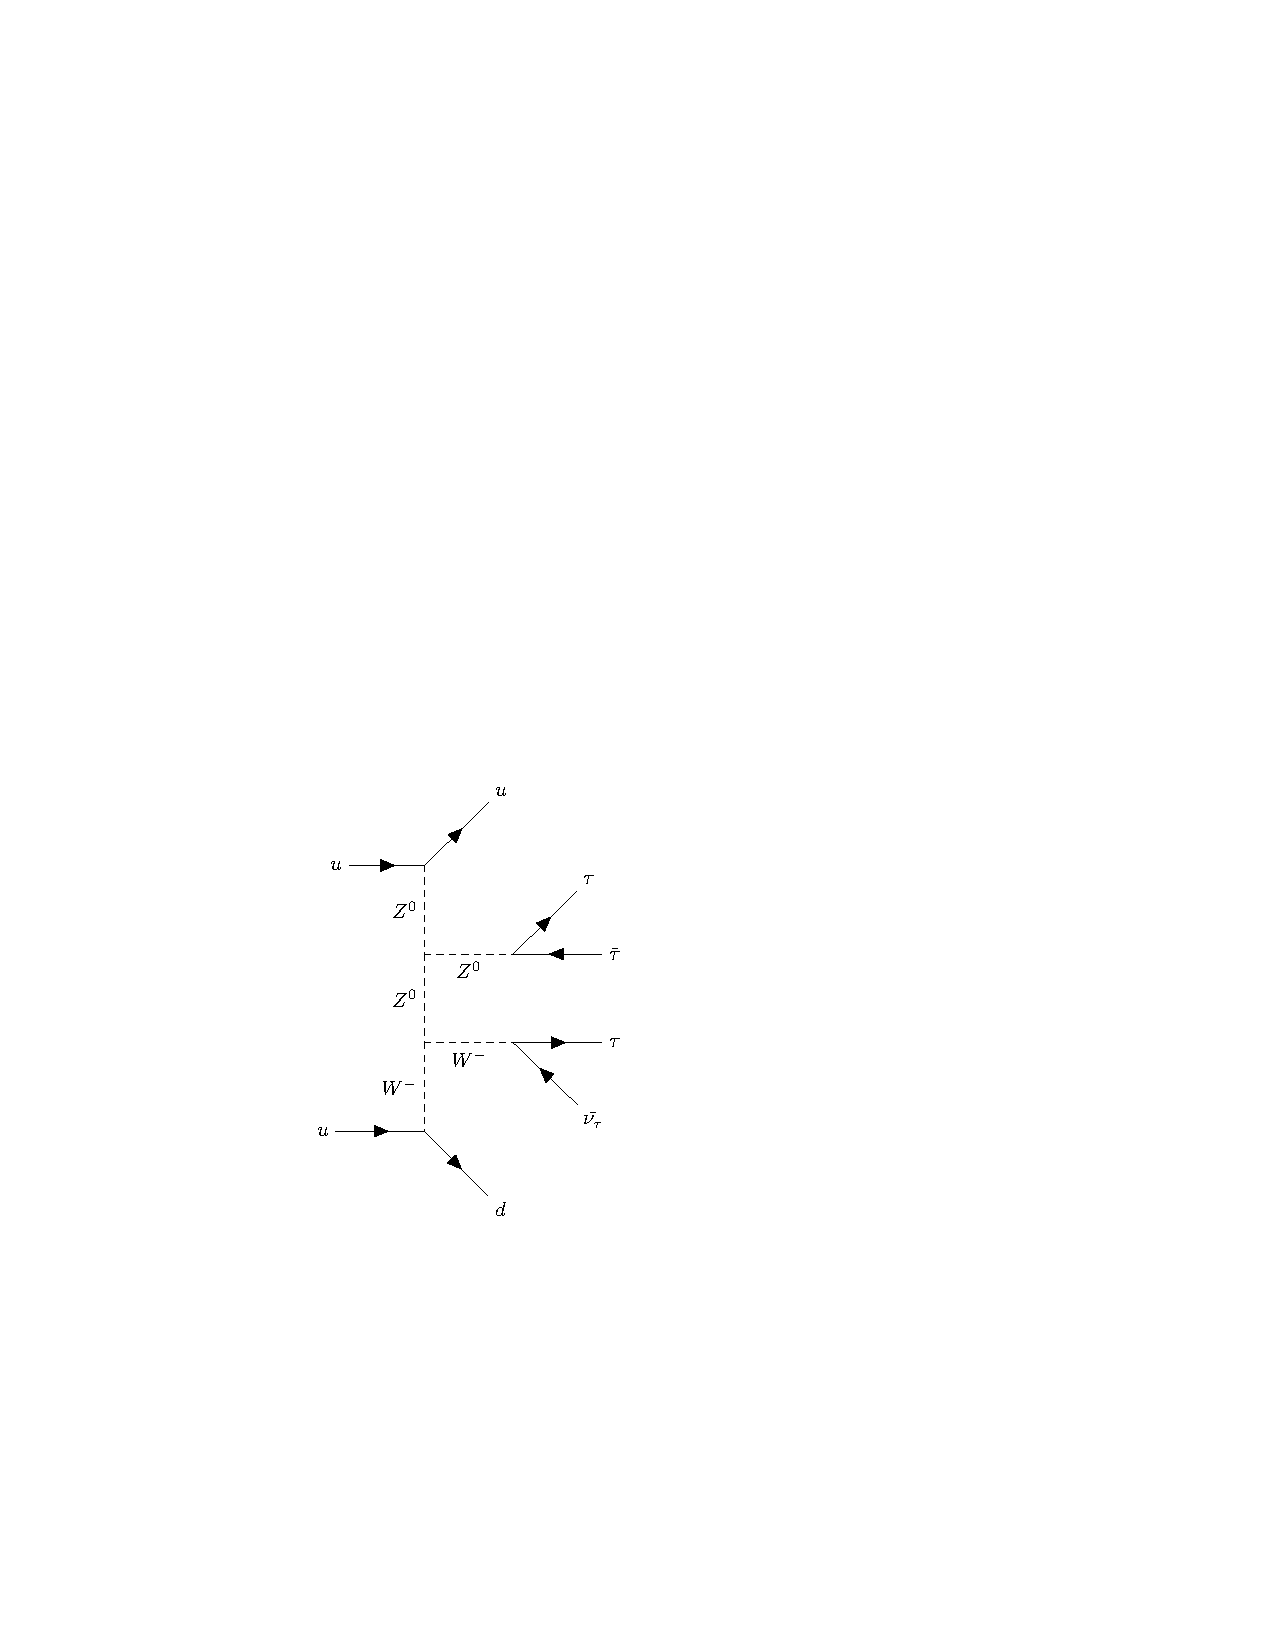
\includegraphics[width=0.48\textwidth]{diagrams/pics/background_SMVBFZ0Wmissminus.pdf}
		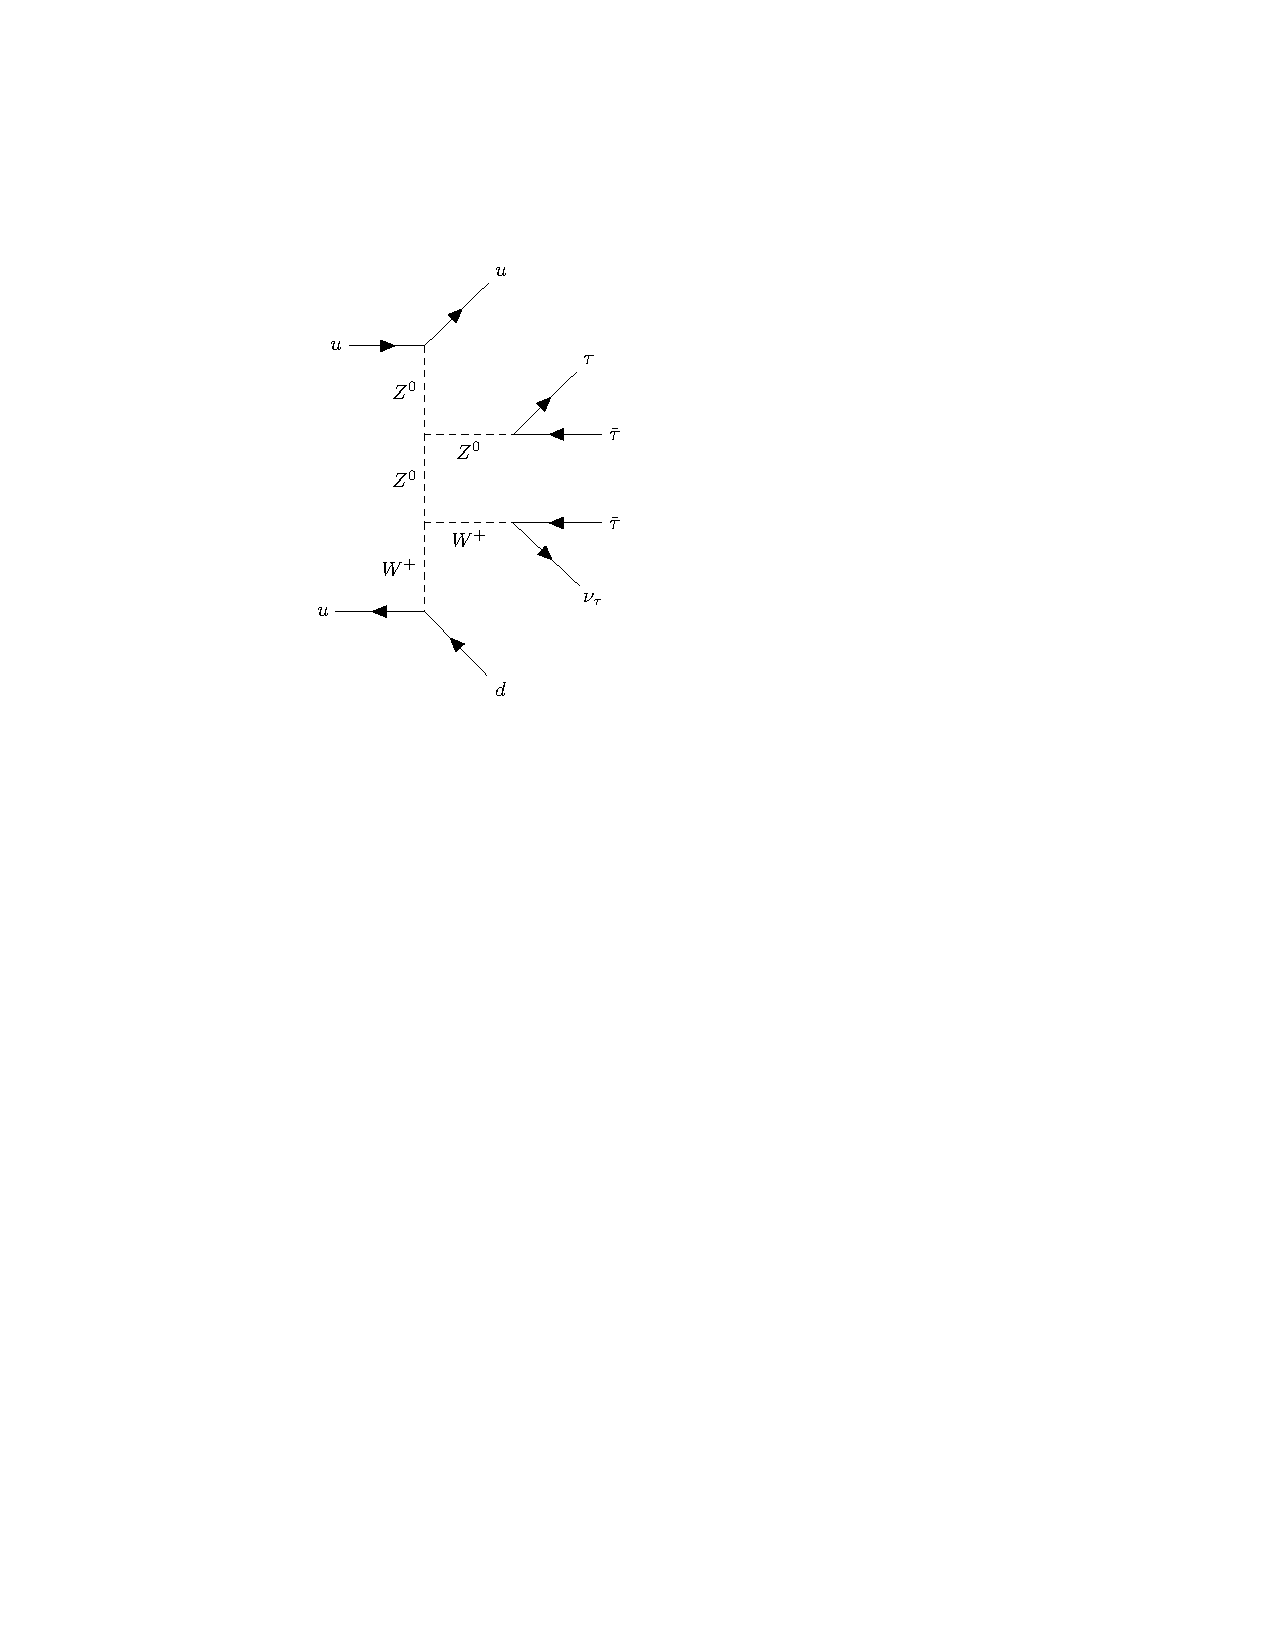
\includegraphics[width=0.48\textwidth]{diagrams/pics/background_SMVBFZ0Wmissplus.pdf} 		
	\end{tabular}
	\caption{Feynman diagrams of irreducible backgrounds of Standard Model Vector Boson  processes ending with three $\tau$ where the opposite charged one fails to pass the tauID selection criteria. }
	\label{fig:background_SMVBFZ0Wmiss}
\end{figure}

Those processes are again purely electroweak, therefore the rate and relative theoretical uncertainty on the rate are small compared to QCD. Additionally, the probability for events coming from this background contribution to pass the event selection is very low. In conclusion, this topology of events is considered to be a minor contribution to the total background.  

Third, there are the Standard Model backgrounds where one of the \hadtau has a mis-reconstructed charge as shown in Figures \ref{fig:background_SMVBFZ0}, \ref{fig:background_SMVBFH} and \ref{fig:background_ttbar}. 

\begin{figure}[tbh!]
	\centering
	\begin{tabular}{cc}
		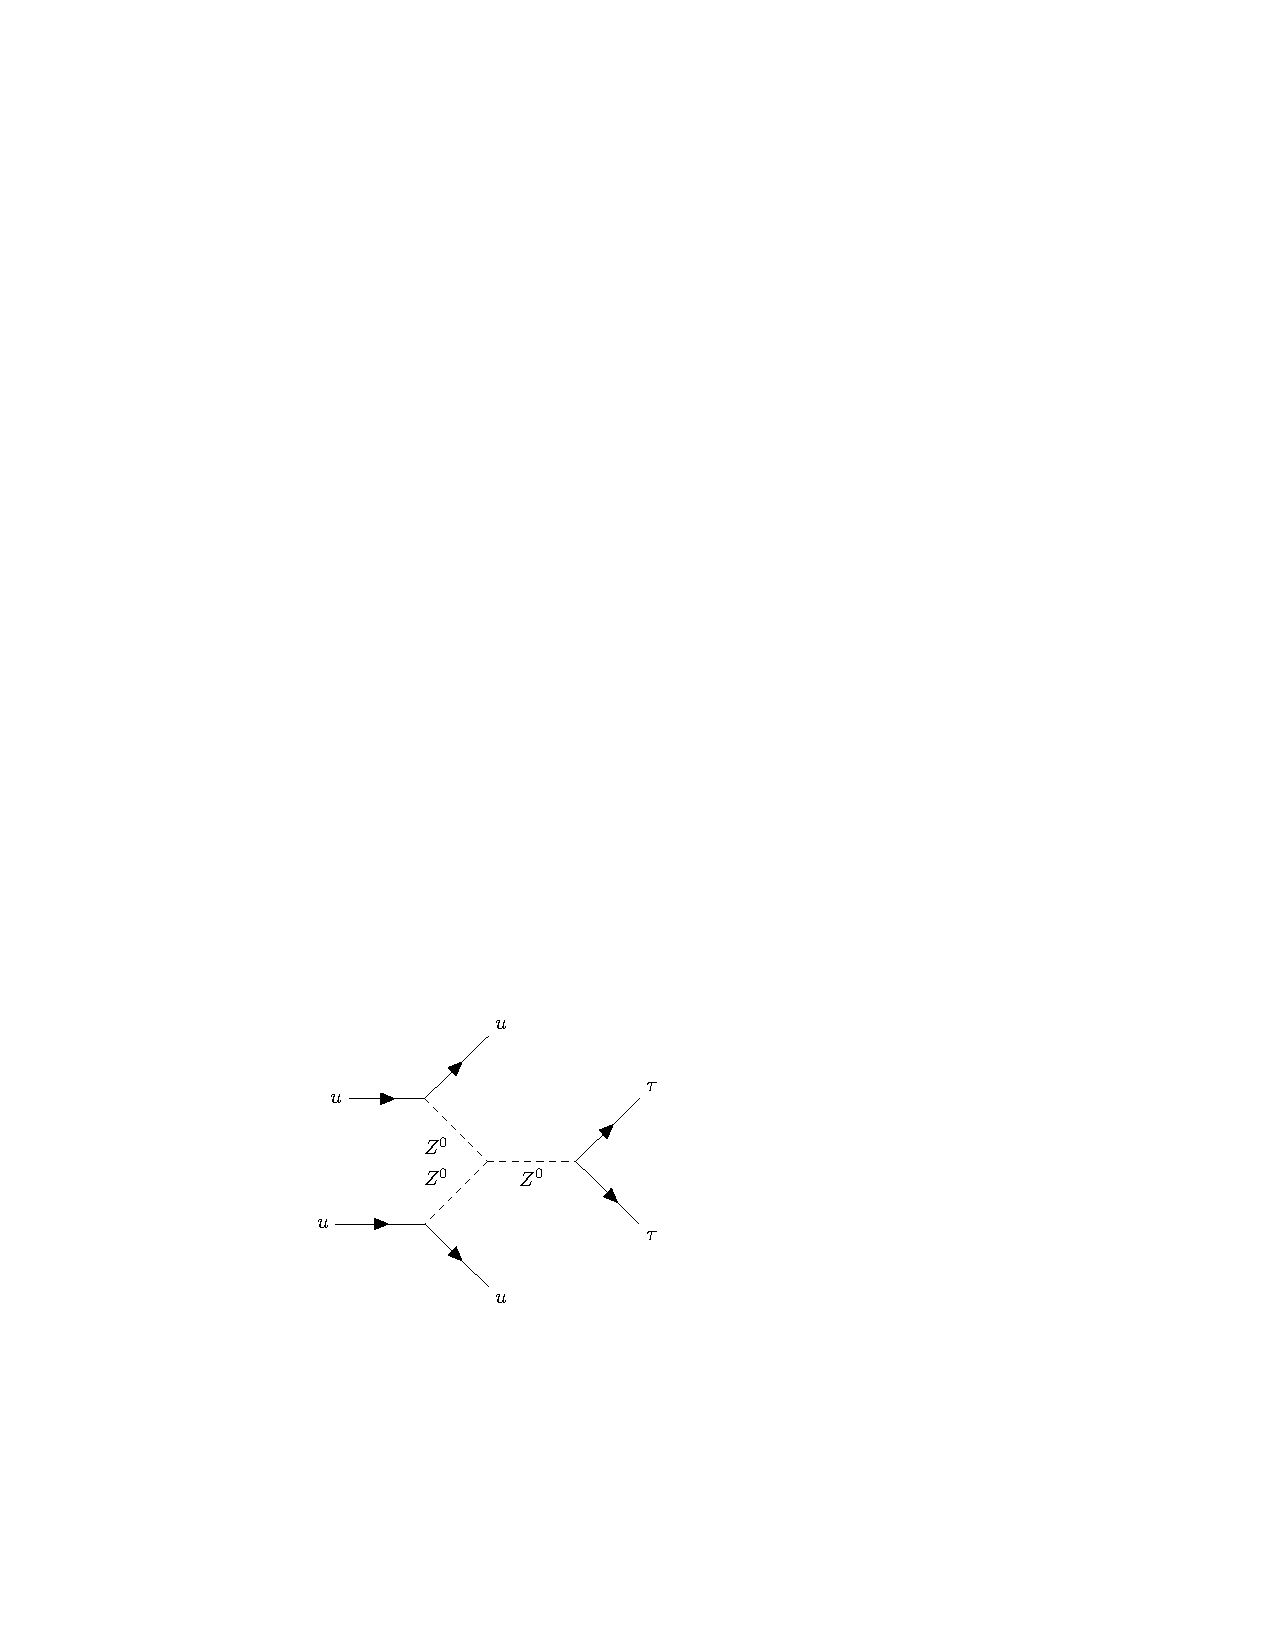
\includegraphics[width=0.48\textwidth]{diagrams/pics/background_SMVBFZ0Z0.pdf}
		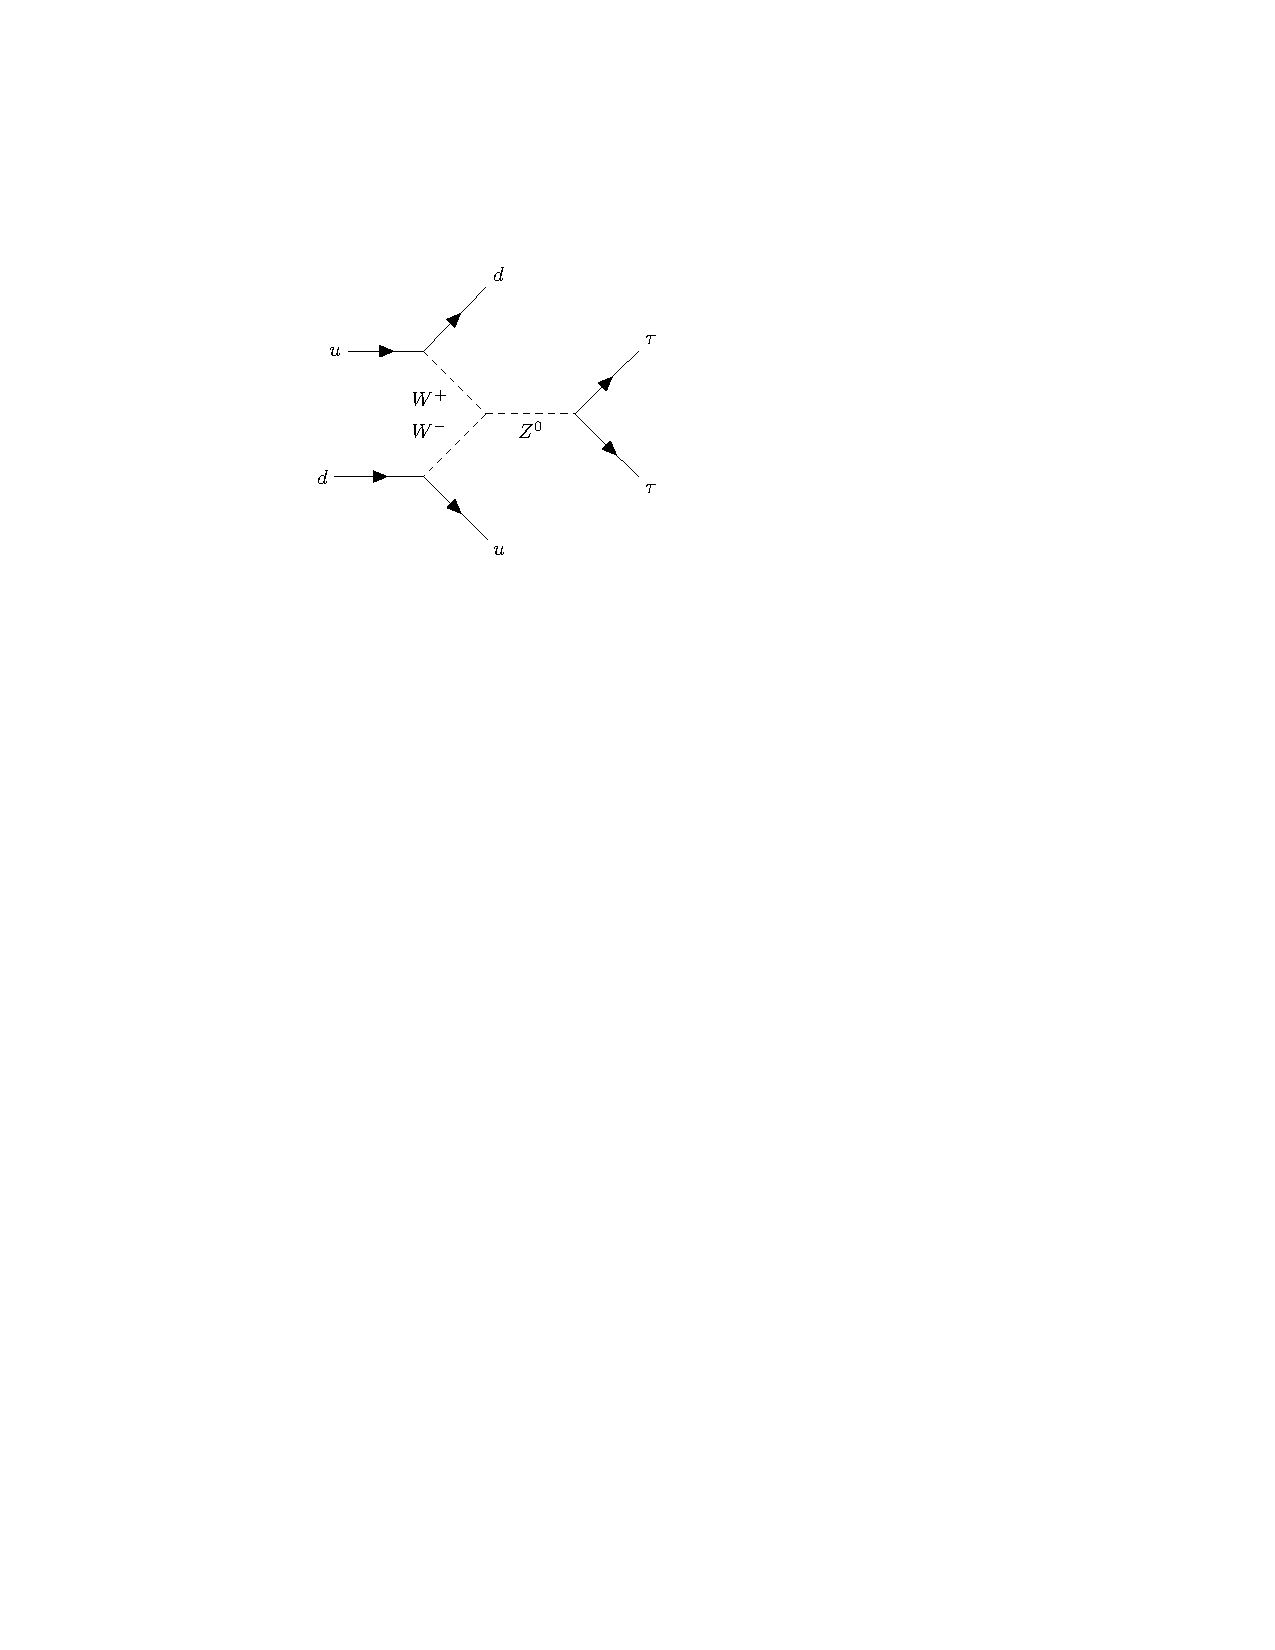
\includegraphics[width=0.48\textwidth]{diagrams/pics/background_SMVBFZ0W.pdf} 		
	\end{tabular}
	\caption{Feynman diagrams of irreducible backgrounds of Standard Model Vector Boson Fusion $Z^{0}$ production. }
	\label{fig:background_SMVBFZ0}
\end{figure}

\begin{figure}[tbh!]
	\centering
	\begin{tabular}{cc}
		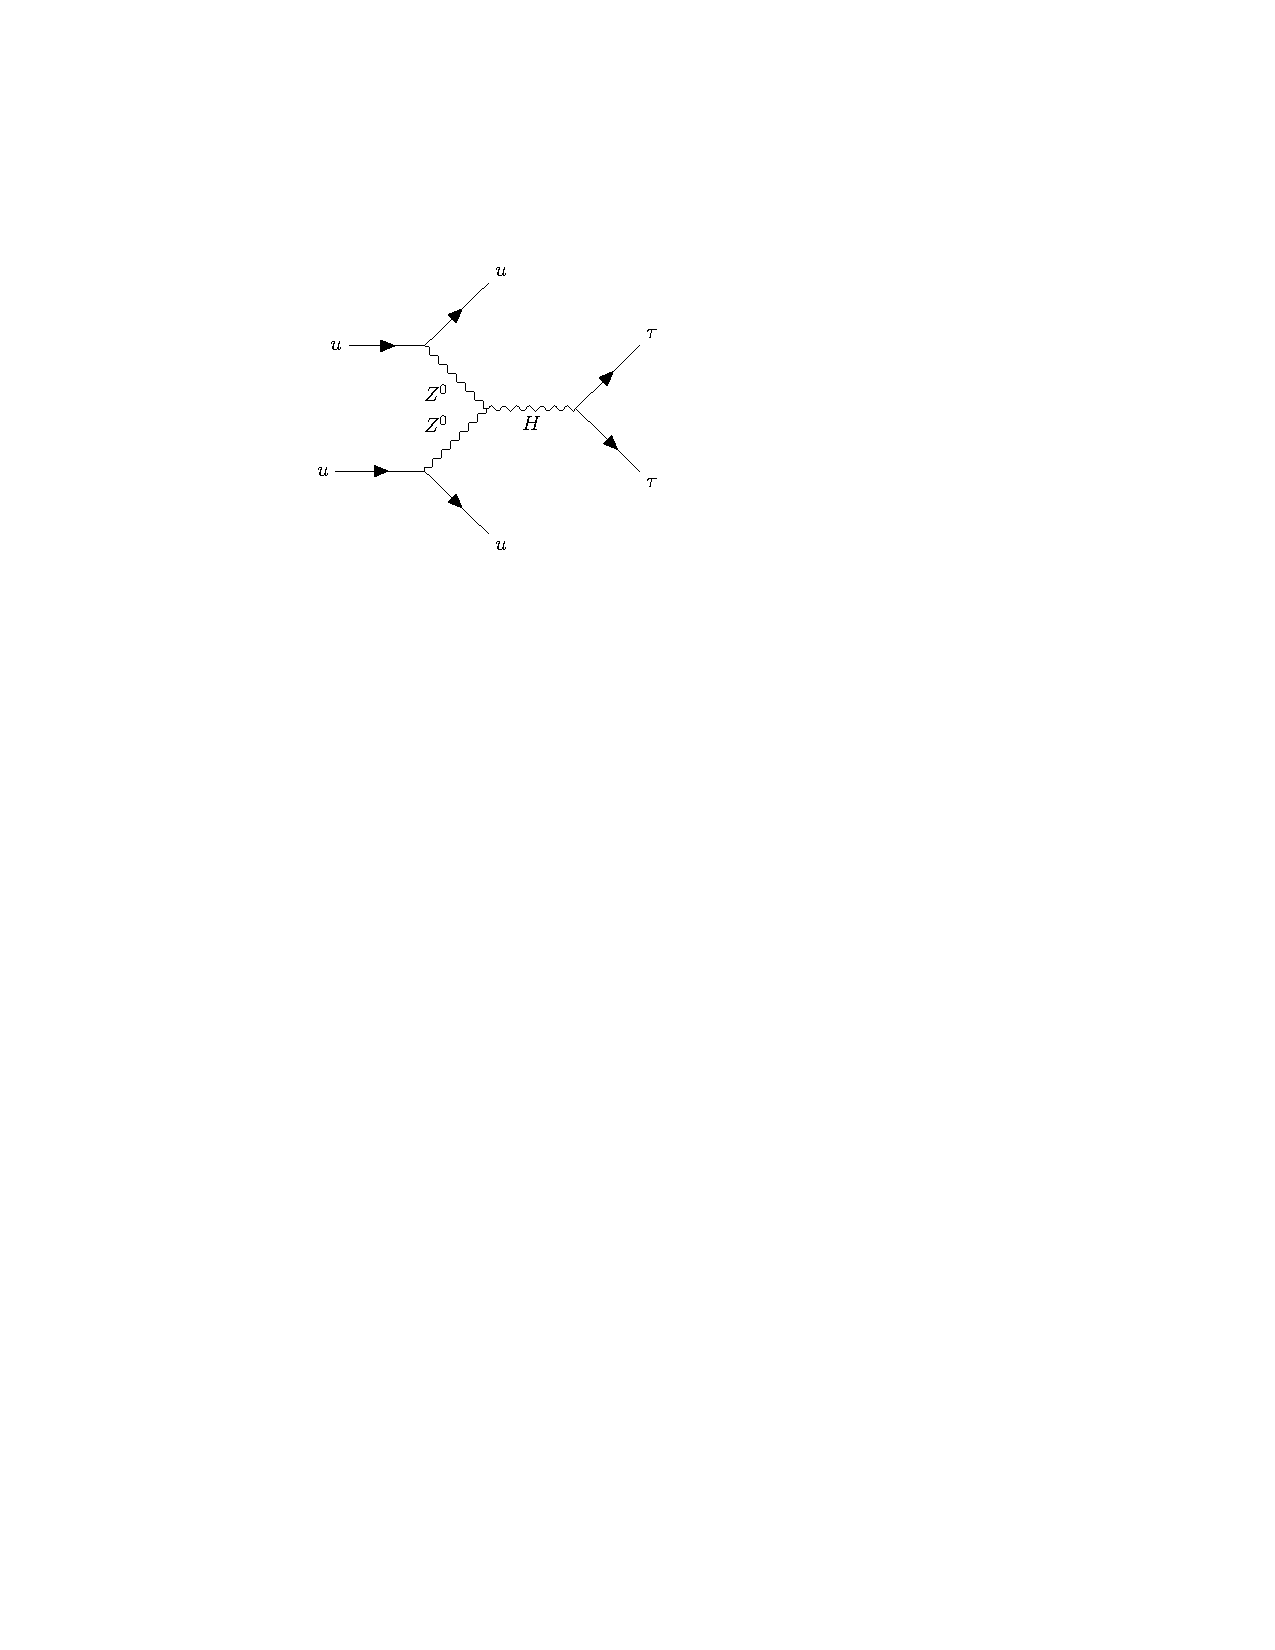
\includegraphics[width=0.48\textwidth]{diagrams/pics/background_HZ0.pdf}
		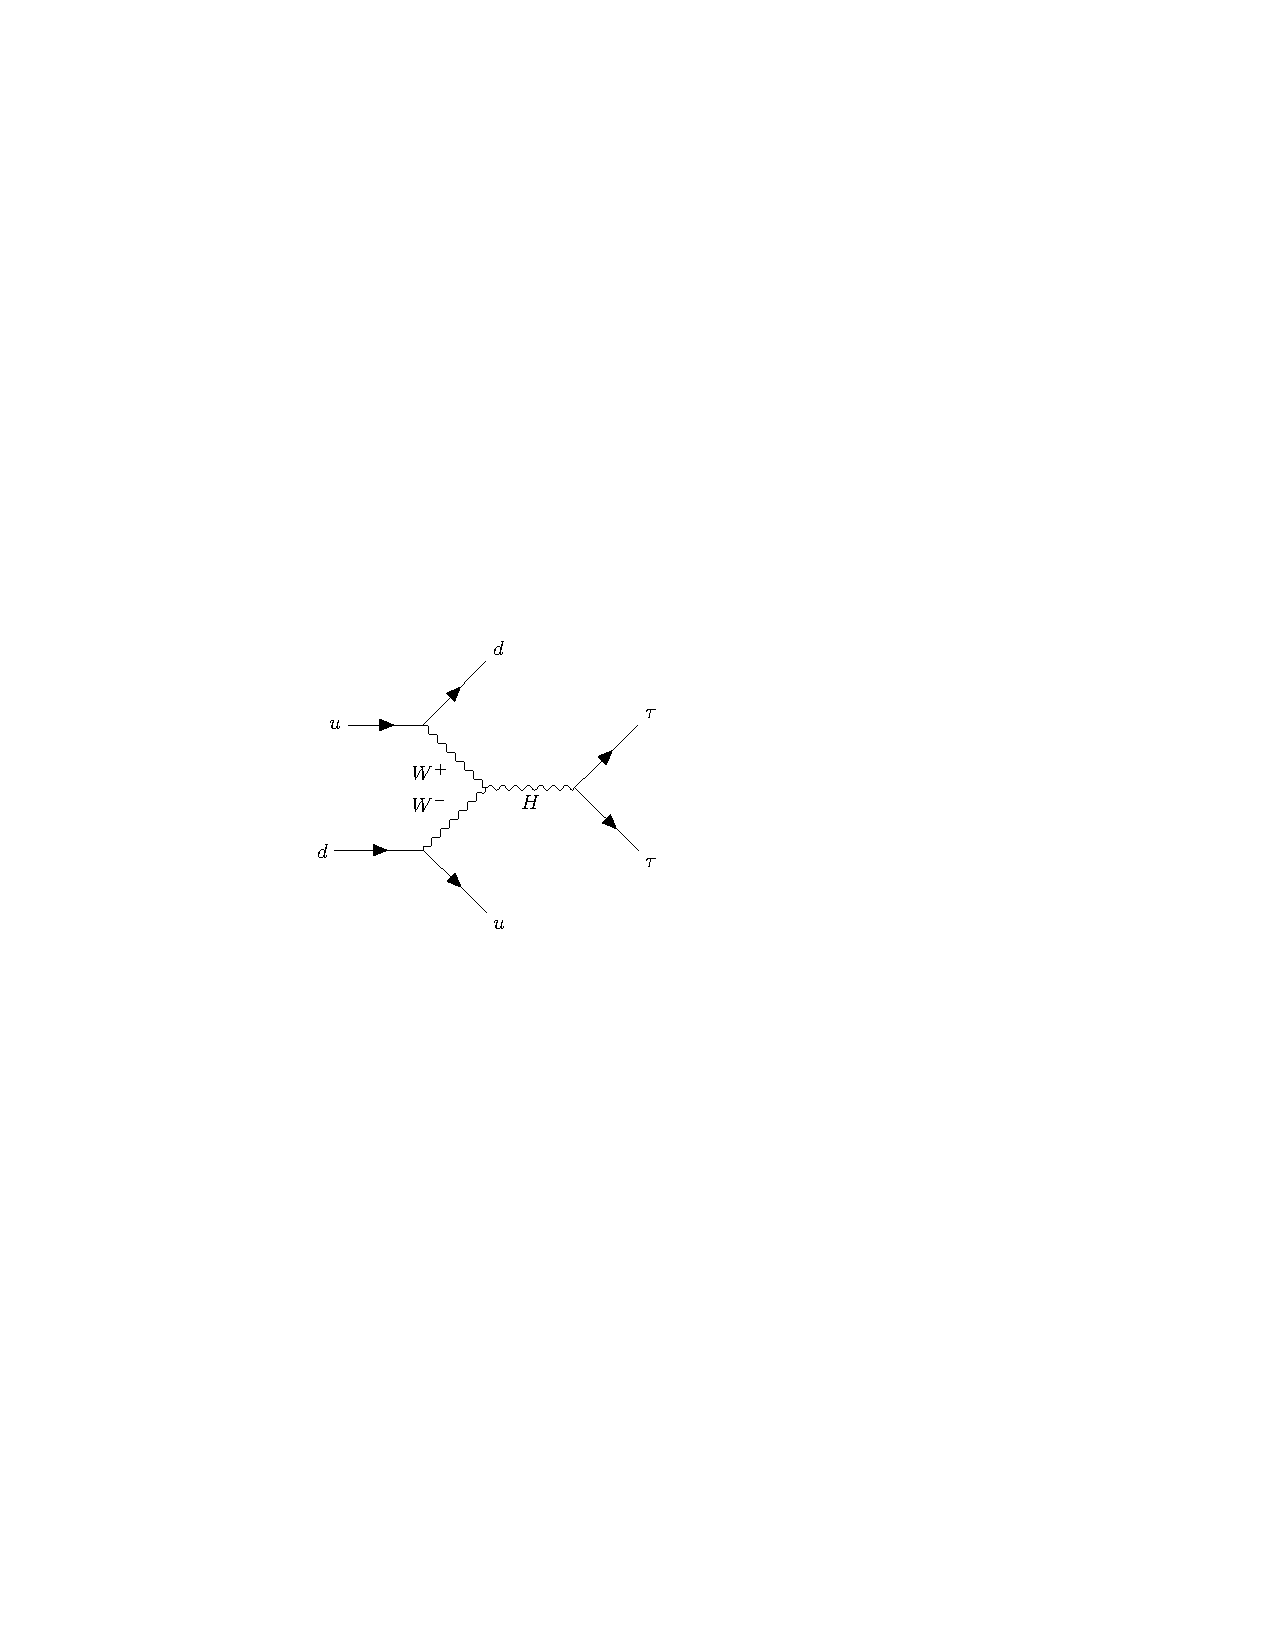
\includegraphics[width=0.48\textwidth]{diagrams/pics/background_HW.pdf} 		
	\end{tabular}
	\caption{Feynman diagrams of irreducible backgrounds of Standard Model Vector Boson Fusion Higgs production. }
	\label{fig:background_SMVBFH}
\end{figure}

\begin{figure}[tbh!]
	\centering
	\begin{tabular}{cc}
		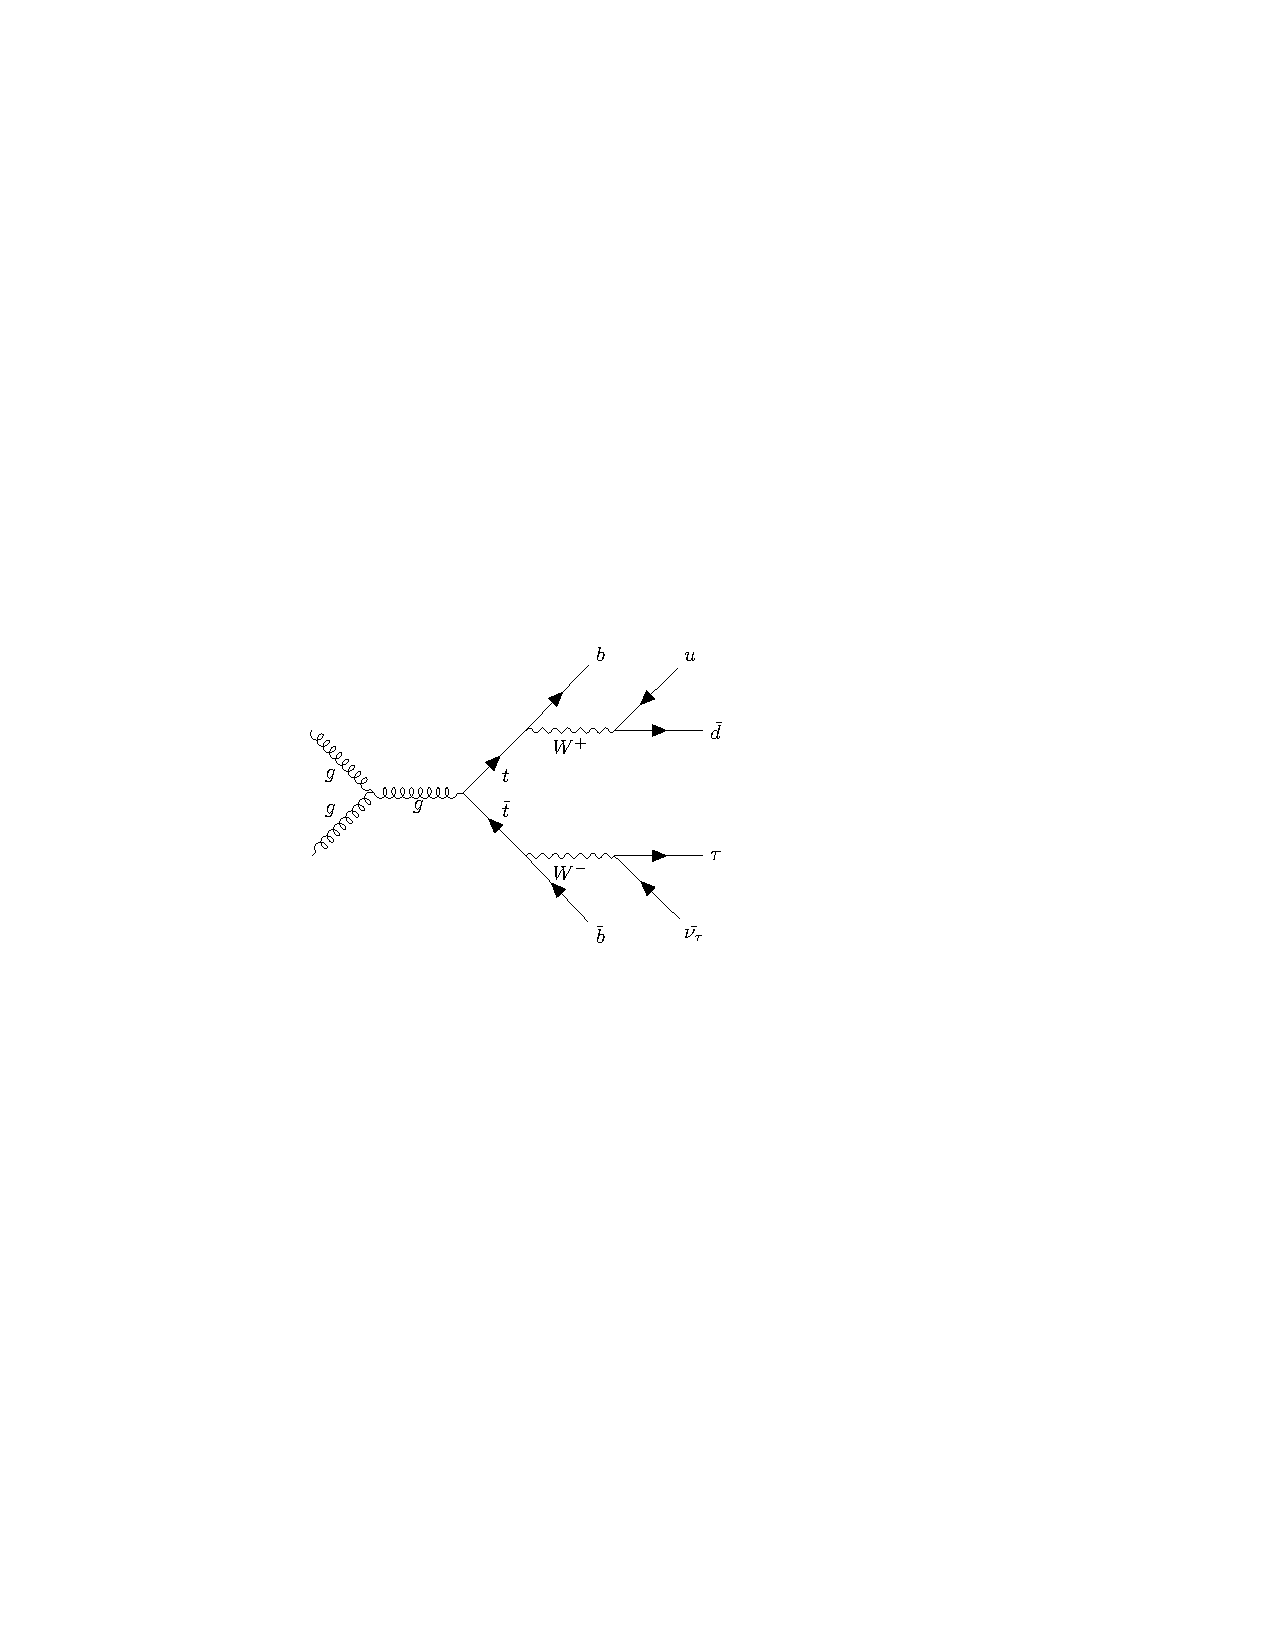
\includegraphics[width=0.75\textwidth]{diagrams/pics/background_ttbar.pdf}
	\end{tabular}
	\caption{\ttbar production is part of background if one of the jets is reconstructed as a \hadtau.}
	\label{fig:background_ttbar}
\end{figure}

All of these processes have a very low cross section compared to the one coming from the main background contribution, therefore those processes are all considered a minor background and their event contribution is taken directly from simulation.

The last background contribution comes from all the QCD events resulting in four jets with two of those jests reconstructed as a fake \hadtau. Even though the probability of a jet to fake a \hadtau is low, the production cross sections of QCD events in a hadron collider are large. Therefore, even small \hadtaufake rates from QCD processes, matter. Also, in QCD events, additional jet activity from initial or final jet radiation processes is expected, which gives these type of events a high probability to pass the VBF selection criteria. Those motivations lead to the determination of QCD as main background source for this analysis. Examples of some QCD processes are shown in Figure \ref{fig:background_QCDinitrad} and \ref{fig:background_QCDfinrad}.

\begin{figure}[tbh!]
	\centering
	\begin{tabular}{cc}
		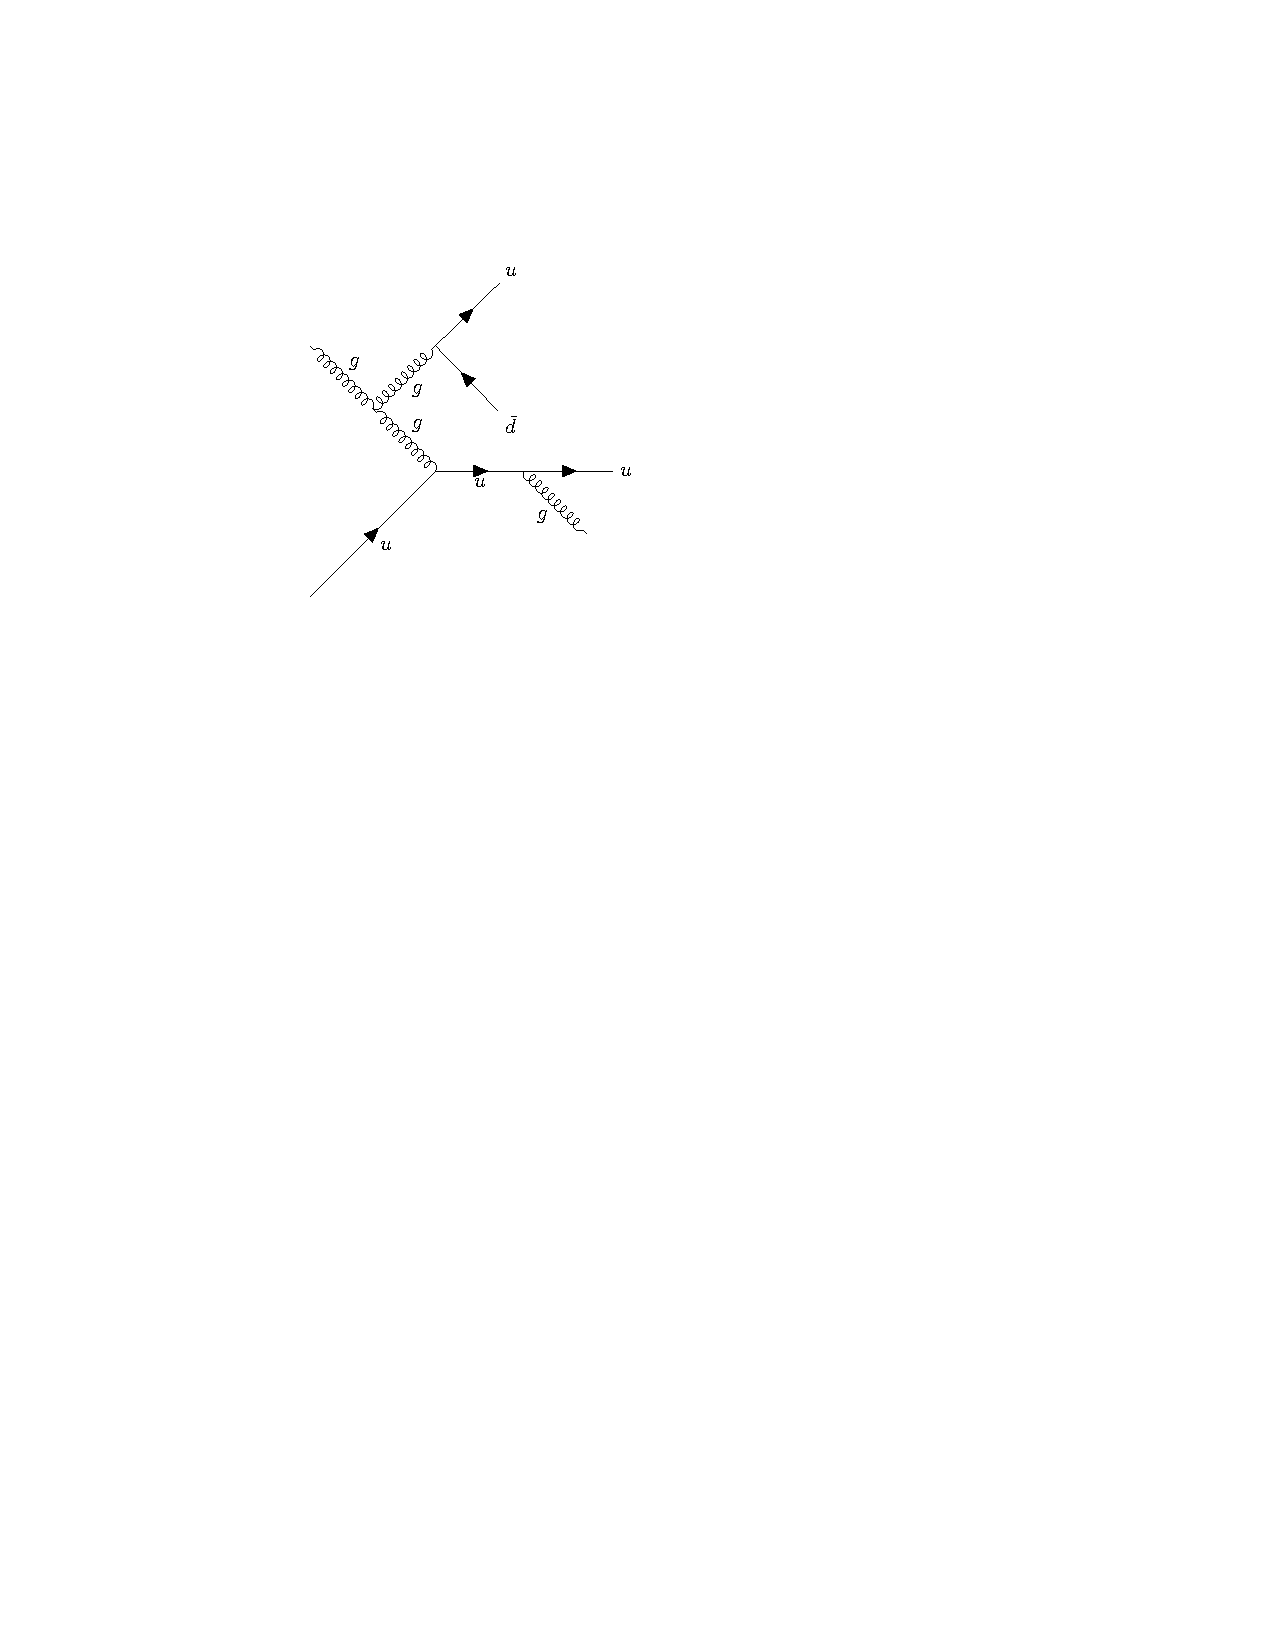
\includegraphics[width=0.75\textwidth]{diagrams/pics/background_QCDinitrad.pdf}
	\end{tabular}
	\caption{Feynman diagrams of a four jet QCD prodution with initial state radiation where two jets are misreconstructed as \hadtau. }
	\label{fig:background_QCDinitrad}
\end{figure}

\begin{figure}[tbh!]
	\centering
	\begin{tabular}{cc}
		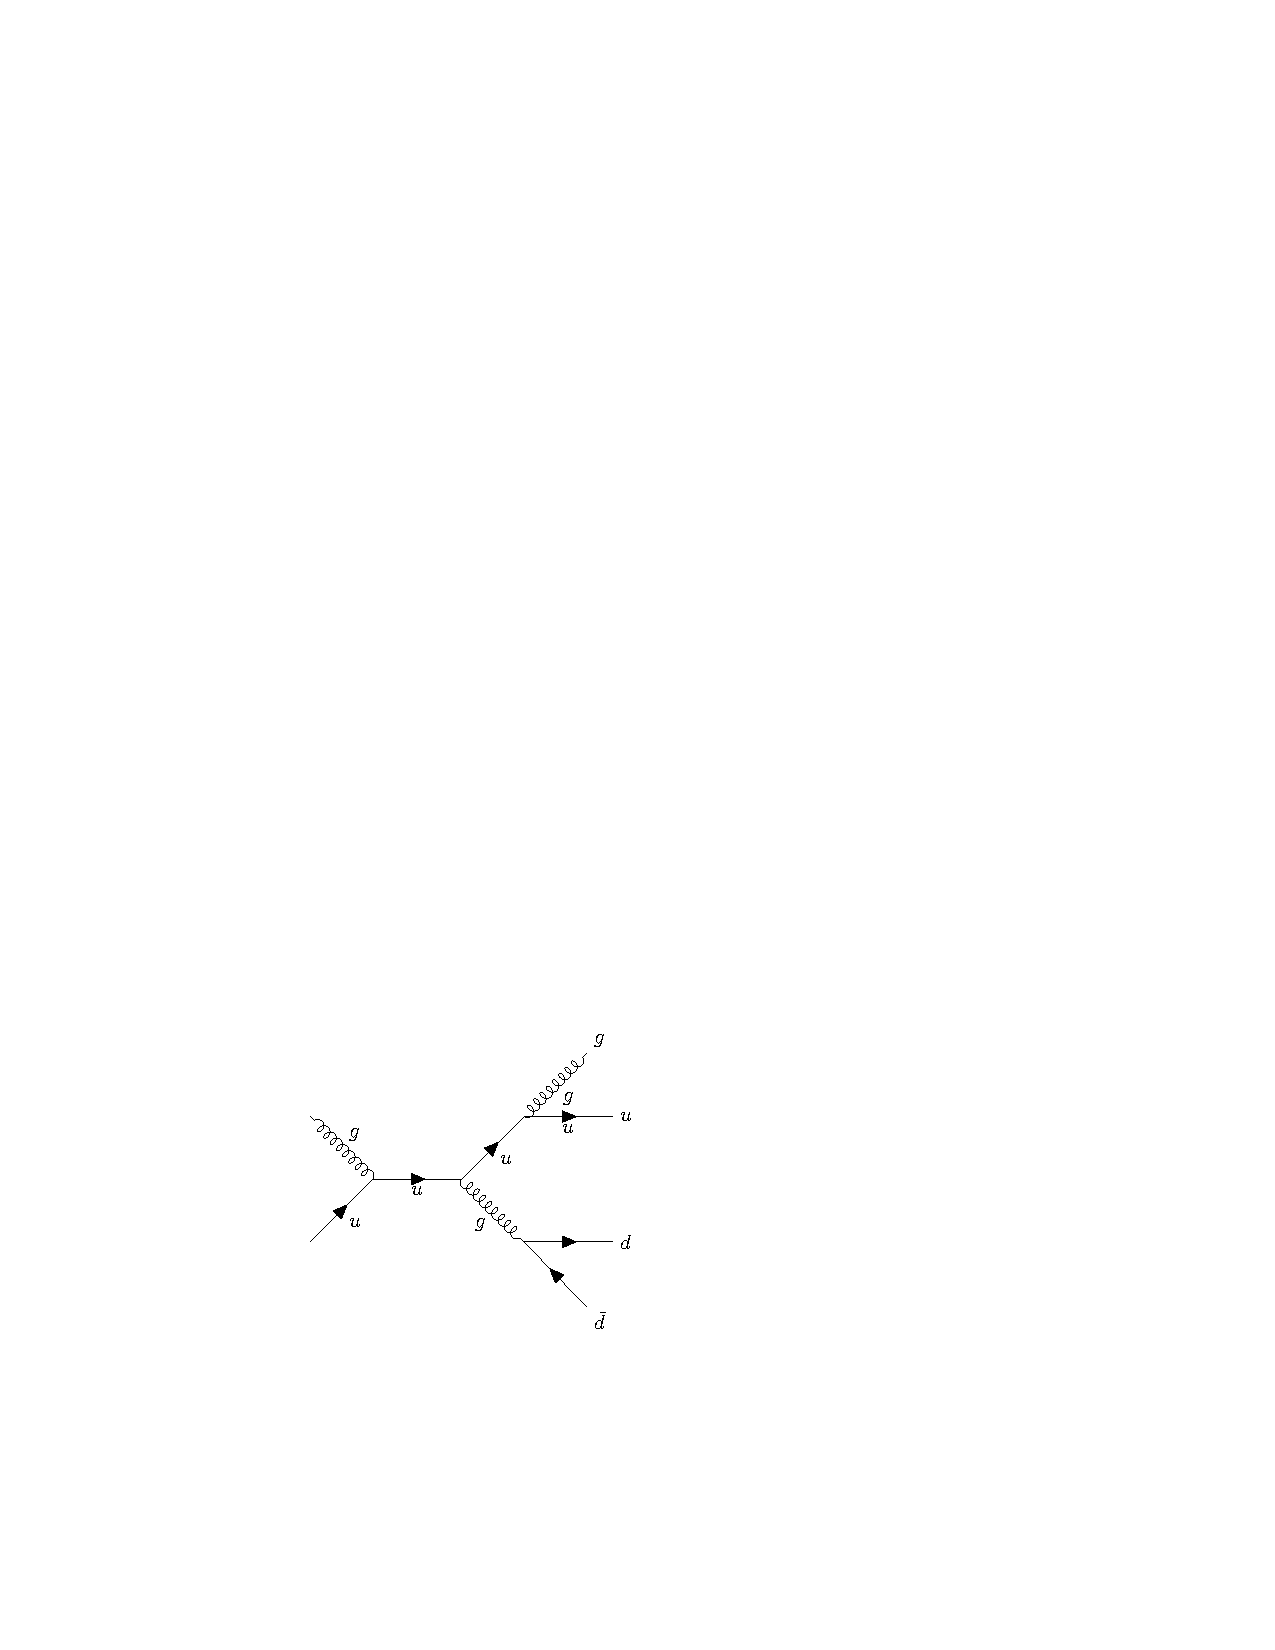
\includegraphics[width=0.75\textwidth]{diagrams/pics/background_QCDfinrad.pdf}
	\end{tabular}
	\caption{Feynman diagrams of a 4 jet QCD prodution with final state radiation where two jets are misreconstructed as \hadtau. }
	\label{fig:background_QCDfinrad}
\end{figure}

Similarly to the processes described before there are QCD processes resulting in one \hadtau and three jets with one of the jets mis-reconstructed as the second \hadtau. Examples of those processes are shown on Figure \ref{fig:background_W3jets}

\begin{figure}[tbh!]
	\centering
	\begin{tabular}{cc}
		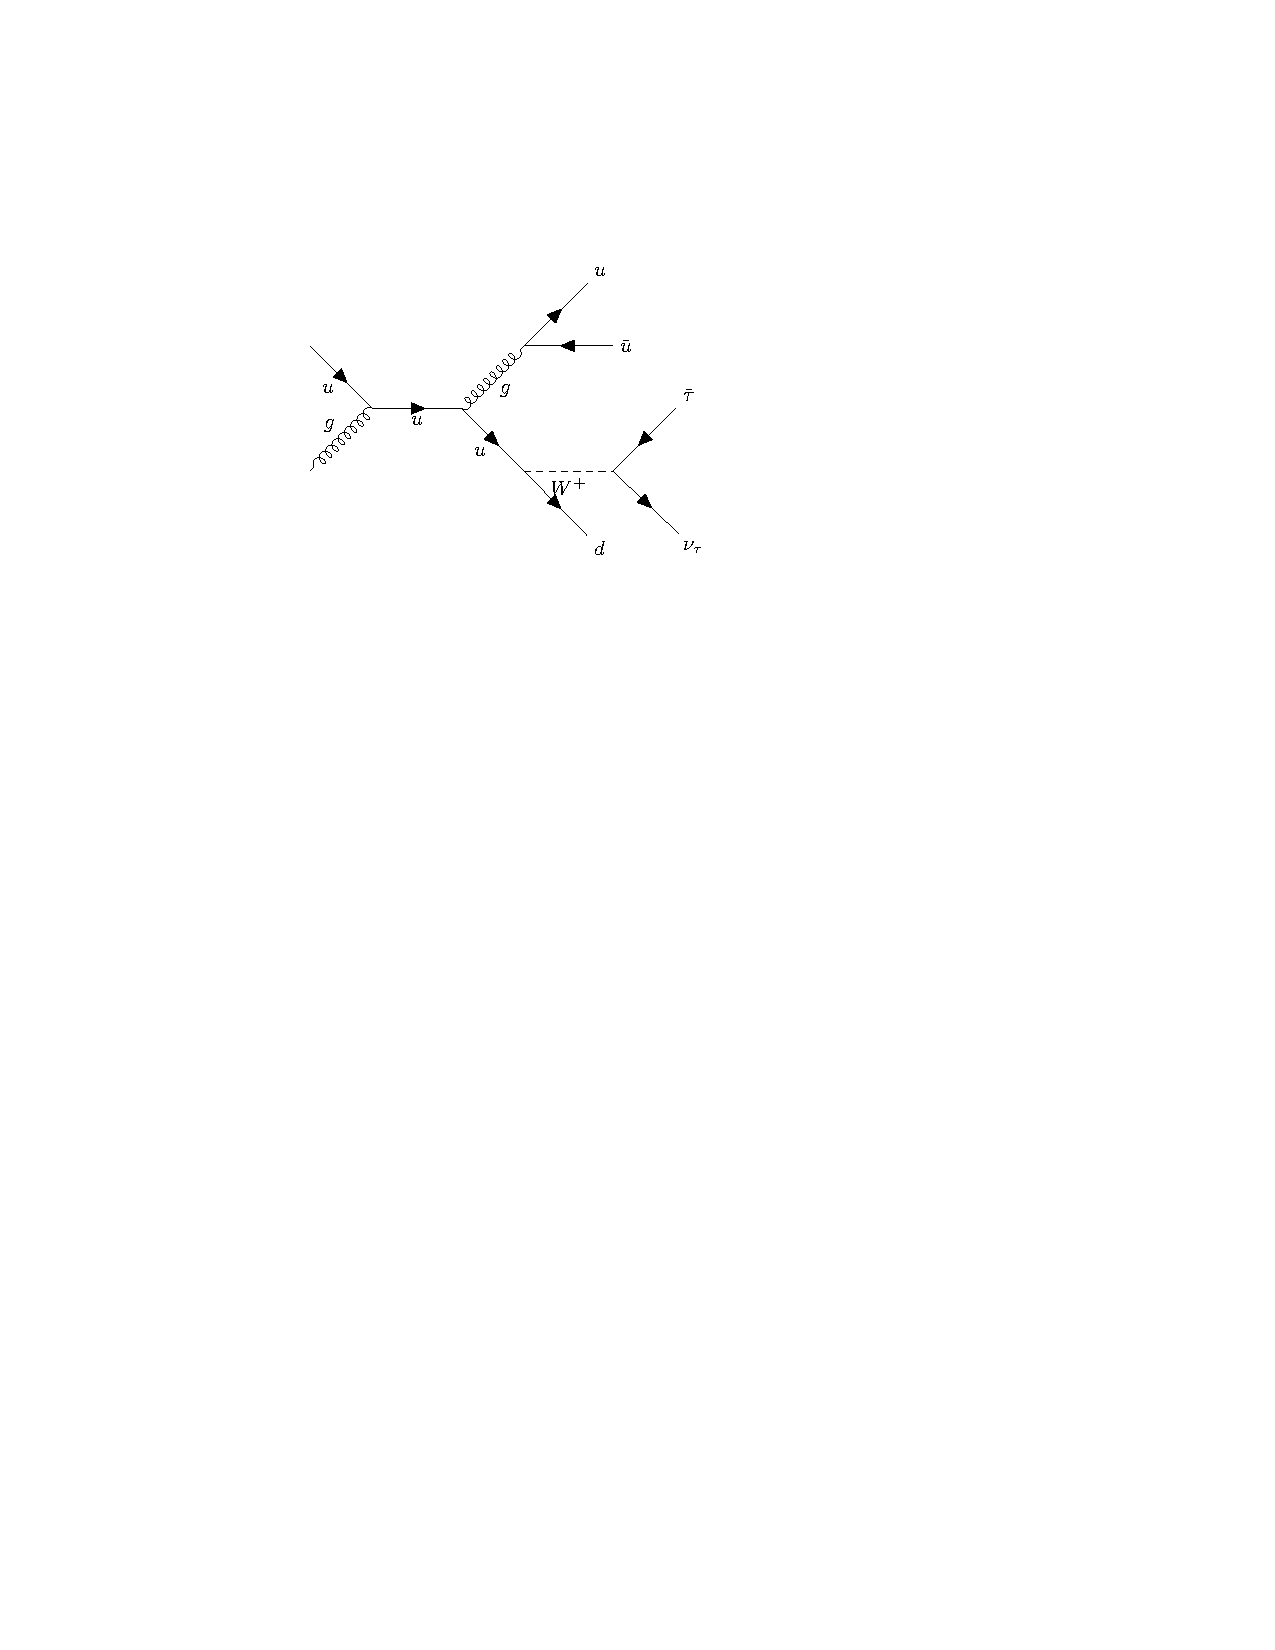
\includegraphics[width=0.75\textwidth]{diagrams/pics/background_W3jets.pdf}
	\end{tabular}
	\caption{Feynman diagrams of W boson plus 3 jets production where one jet is mis-reconstructed as \hadtau. }
	\label{fig:background_W3jets}
\end{figure}

\begin{figure}[tbh!]
	\centering
	\begin{tabular}{cc}
		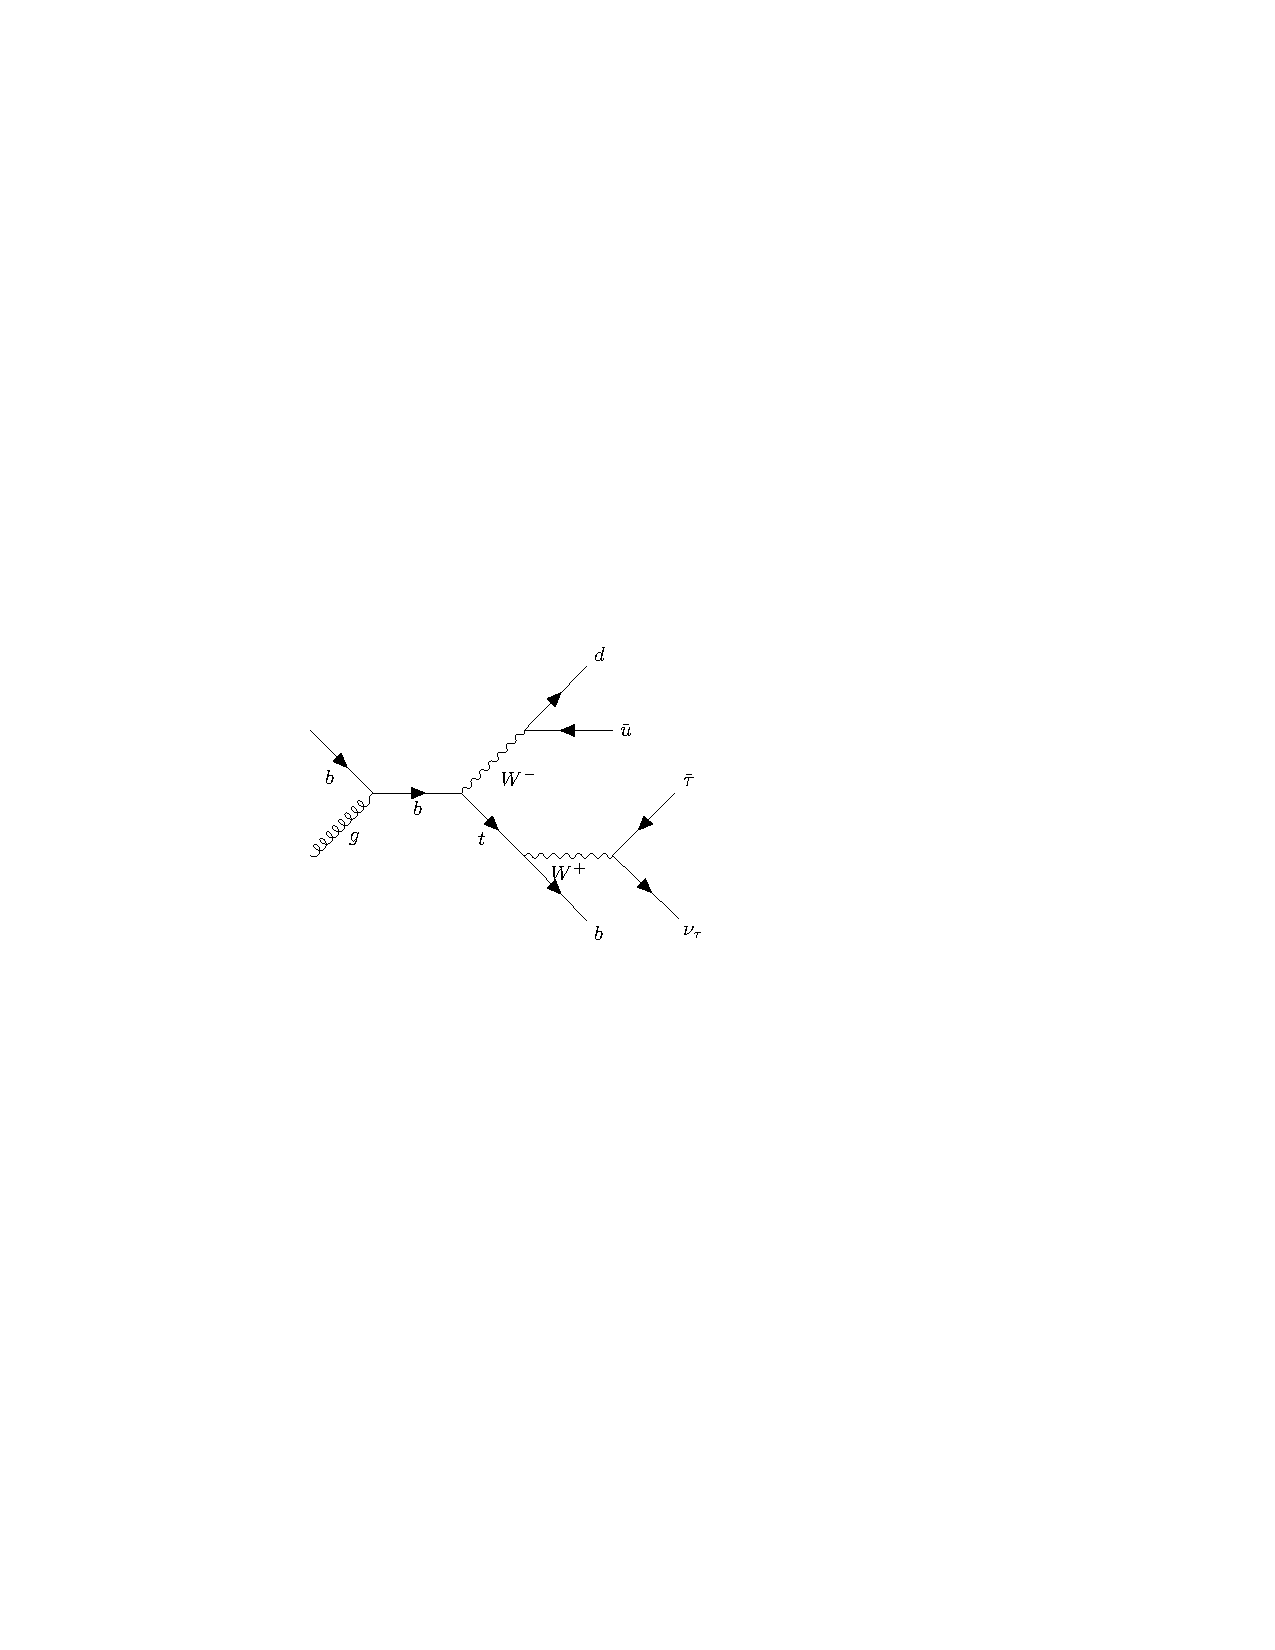
\includegraphics[width=0.75\textwidth]{diagrams/pics/background_singlet.pdf}
	\end{tabular}
	\caption{Feynman diagrams of single top production where one jet is mis-reconstructed as \hadtau. }
	\label{fig:background_singlet}
\end{figure}

\clearpage
